\documentclass{article}

\usepackage[a4paper,margin=2cm]{geometry}
\usepackage{graphicx}

%% Hack the caption:
%% http://tex.stackexchange.com/questions/41597/remove-colon-in-the-caption-of-a-figure-without-using-caption-package

\usepackage{url,booktabs}
%%\usepackage{etoolbox}
%% \makeatletter
%% \patchcmd{\@makecaption}{#1: #2}{\textbf{#1} #2}{}{}
%% \makeatother



% !!! For some reason it complains about one of the captions, wants to
% add a $ sign...??

\begin{document}
\pagestyle{empty}


%% http://bytesizebio.net/2013/03/11/adding-supplementary-tables-and-figures-in-latex/
\newcommand{\beginsupplement}{%
  \setcounter{table}{0}
  \renewcommand{\thetable}{S\arabic{table}}%
  \setcounter{figure}{0}
  \renewcommand{\thefigure}{S\arabic{figure}}%
}

\beginsupplement

% !!!
% Generated using drawAllNeurons.m
%

\begin{figure}
  \centering
  \fbox{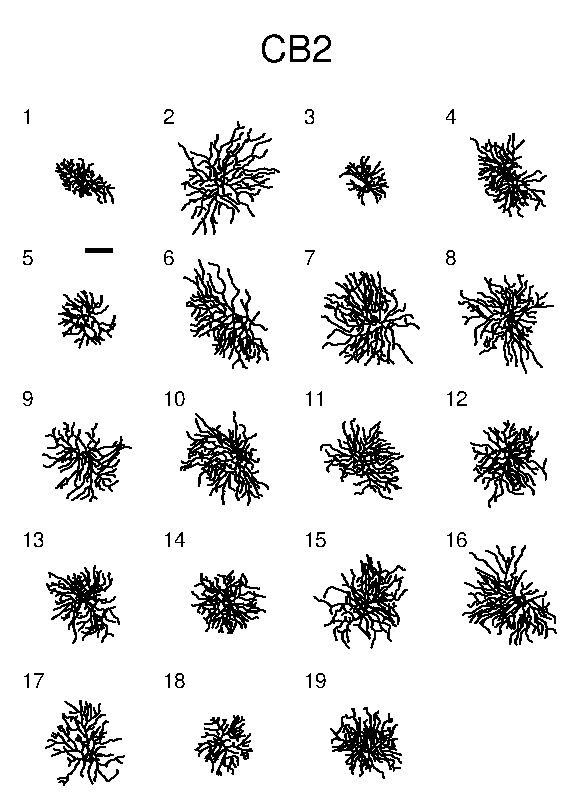
\includegraphics[scale=1]{Figures/SupFig1/CB2-all-cells-1.eps}}
  \caption{}
\end{figure}

\begin{table}
  \centering
  \begin{tabular}{rl}
    \toprule
    cell & file \\
    \midrule
    1& \url{CB2-06142012-cell1-40x}  \\
2& \url{CB2-06202012-new}  \\
3& \url{CB2-06222012-cell2-b-corrected}  \\
4& \url{CB2-07182012-r1-cell1-40x-06zoom-corrected}  \\
5& \url{CB2-07182012-r1-cell3-40x-0-corrected}  \\
6& \url{CB2-2ears-R1-07062012-cell1-40x-stitch}  \\
7& \url{CB2-2ears-R1-07062012-cell3-40x-06zoom}  \\
8& \url{CB2-2ears-R1-07062012-cell4-40x-06zoom}  \\
9& \url{CB2-2ears-R2-07062012-cell1-40x-06zoom}  \\
10& \url{CB2-P62-06252012-40x-stitch}  \\
11& \url{CB2-T4-R1-07092012-cell2-40x-stitch}  \\
12& \url{CB2-T4-R2-07092012-cell1-40x-stitch}  \\
13& \url{CB2-T4-R2-07092012-cell2-40x-07zoom}  \\
14& \url{CB2-T4-R2-07092012-cell3-40x-08zoom}  \\
15& \url{CB2-nomark-R1-beads-07042012-cell1-40x-06zoom}  \\
16& \url{CB2-rightear-R1-beads-07032012-cell1-40x-06zoom}  \\
17& \url{CB2-rightear-R2-beads-07032012-cell1-40x-07zoom}  \\
18& \url{P61-CB2-06252012-r2-cell1-40x-grey}  \\
19& \url{P61-CB2-06252012-r2-cell2-40x-b}  \\
\bottomrule
  \end{tabular}
  \caption{CB2 Filenames}
\end{table}

\clearpage

\begin{figure}
  \centering
  \fbox{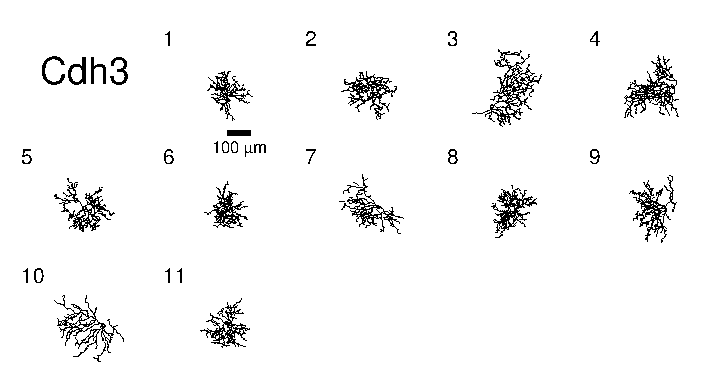
\includegraphics[scale=1.5]{Figures/SupFig1/Cdh3-all-cells-1.eps}}
  \caption{}
\end{figure}

\begin{table}
  \centering
  \begin{tabular}{rl}
    \toprule
    cell & file \\
    \midrule
    1& \url{Cdh3-06112012-corrected} \\
    2& \url{Cdh3-07-17-2012-a2-r2-cell1-40x-0} \\
    3& \url{Cdh3-07-17-2012-a2-r2-cell2-40x-0} \\
    4& \url{Cdh3-07-18-2012--cell1-40x-0-corrected} \\
    5& \url{Cdh3-07-18-2012-a2r2-cell1-40x-0-corrected} \\
    6& \url{Cdh3-07-18-2012-a2r2-cell2-40x-corrected} \\
    7& \url{Cdh3-07172012-a1r1-cell1-40x-0} \\
    8& \url{Cdh3-07172012-a3r3-cell1-40x-09zoom-2} \\
    9& \url{Cdh3-07172012-a3r3-cell2-40x-0} \\
    10& \url{Cdh3-a3r3-07172012-cell3-40x-0} \\
    11& \url{cdh3-03122012-corrected} \\
    \bottomrule
  \end{tabular}
\end{table}



\clearpage

\begin{figure}
  \centering
  \fbox{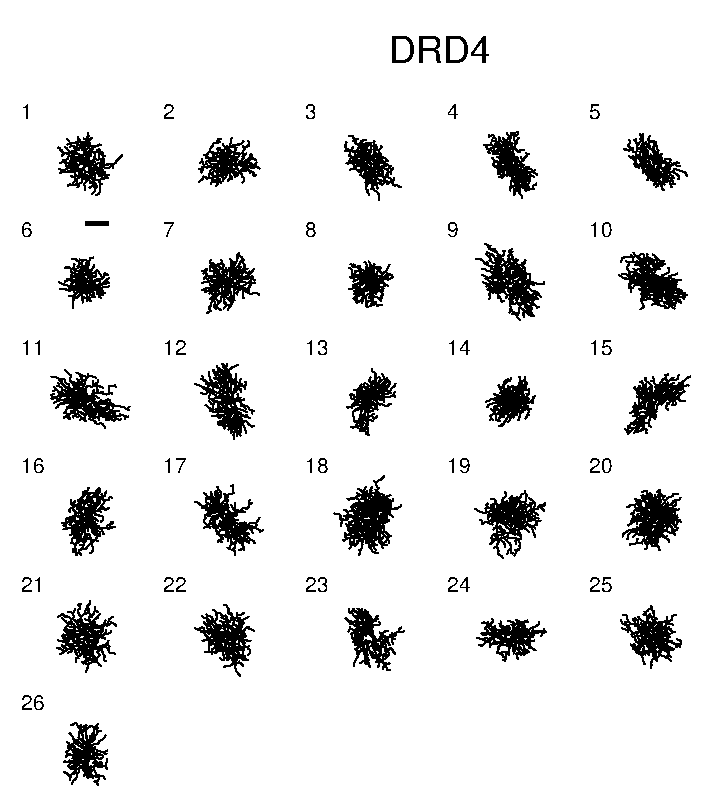
\includegraphics[scale=1.5]{Figures/SupFig1/DRD4-all-cells-1.eps}}
  \caption{}
\end{figure}

\begin{table}
  \centering
  \begin{tabular}{rl}
    \toprule
    cell & file \\
    \midrule
1& \url{DRD4-07142012-r2-cell1-40x-0} \\
2& \url{DRD4-07142012-r2-cell2-40x-0} \\
3&
\url{DRD4-albino-leftearclip-righteye-control-06022013-cell1-40x-07zoom} \\
4&
\url{DRD4-albino-leftearclip-righteye-control-06022013-cell2-40x-07zoom} \\
5&
\url{DRD4-albino-leftearclip-righteye-control-06022013-cell3-40x-0_Subset} \\
6&
\url{DRD4-albino-leftearclip-righteye-control-06022013-cell4-40x-09zoom} \\
7&
\url{DRD4-albino-leftearclip-righteye-control-06022013-cell5-40x-08zoom} \\
8& \url{DRD4-albino-leftearclip-righteye-control-06022013-cell6-40x} \\
9&
\url{DRD4-brown-noearclip-righteye-control-06012013-cell1-40x-06zoom} \\
10&
\url{DRD4-brown-noearclip-righteye-control-06012013-cell2-40x-07zoom} \\
11&
\url{DRD4-brown-noearclip-righteye-control-06012013-cell3-40x-06zoom} \\
12&
\url{DRD4-brown-noearclip-righteye-control-06012013-cell4-40x-tile} \\
13& \url{DRD4-noearclip-righteye-control-06012013-cell1-40x-07zoom} \\
14& \url{DRD4-noearclip-righteye-control-06012013-cell2-40x-09zoom} \\
15& \url{DRD4-noearclip-righteye-control-06012013-cell4-40x-07zoom} \\
16& \url{DRD4-noearclip-righteye-control-06012013-cell5-40x-07zoom} \\
17& \url{DRD4-noearclip-righteye-control-06012013-cell6-40x-07zoom} \\
18& \url{P25-DRD4-07142012-r1-c1-40x-06zoom-grey-corrected} \\
19& \url{P25-DRD4-07142012-r1-c2-40x-07zoom} \\
20& \url{P25-DRD4-07142012-r1-cells3} \\
21& \url{P25-DRD4-07142012-r1-cells4} \\
22& \url{P30-DRD4-07102012-a1r1-cell2-40x-0} \\
23& \url{P30-DRD4-07102012-a1r3-cell1-40x-0} \\
24& \url{P30-DRD4-07102012-a2r1-cell1-40x-07zoom} \\
25& \url{P30-DRD4-07102012-a2r2-cell1-40x-08zoom-grey} \\
26& \url{P30-DRD4-0710210-a1r1-cell1-40x-08zoom} \\
\bottomrule
  \end{tabular}
\end{table}

\clearpage

\begin{figure}
  \centering
  \fbox{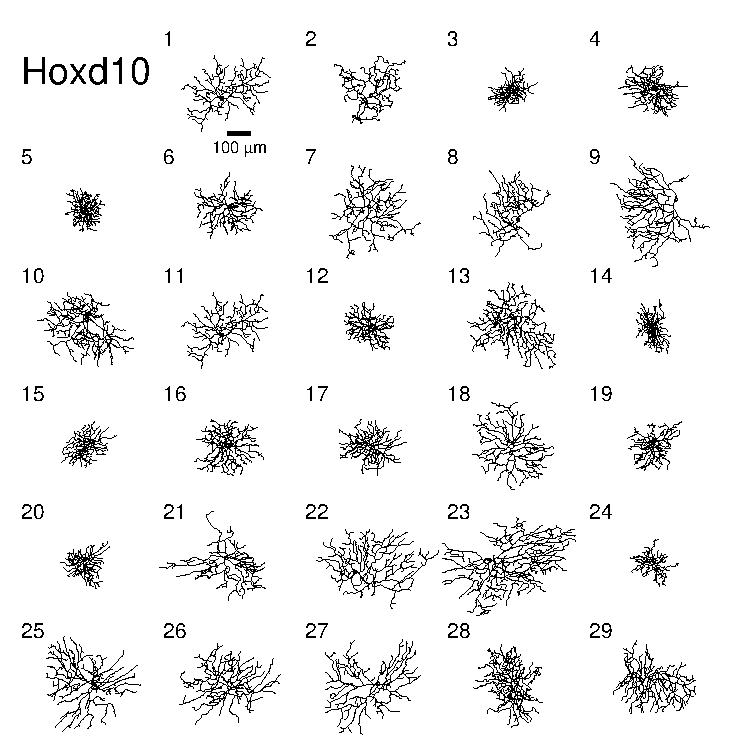
\includegraphics[scale=1.5]{Figures/SupFig1/Hoxd10-all-cells-1.eps}}
  \caption{}
\end{figure}

\begin{table}
  \centering
  \begin{tabular}{rl}
    \toprule
    cell & file \\
    \midrule
1& \url{Hoxd10-02242012} \\
2& \url{Hoxd10-03122012-c1-corrected} \\
3& \url{Hoxd10-03122012} \\
4& \url{Hoxd10-03132012-r1c3-corrected} \\
5& \url{Hoxd10-04022012} \\
6& \url{Hoxd10-04032012-corrected} \\
7& \url{Hoxd10-04292013-leftear-righteyecontrol-cell3-40x-tile_Stitch} \\
8&
\url{Hoxd10-04292013-rightear-righteyecontrol-cell1-40x-tile_Stitch} \\
9& \url{Hoxd10-04292013-rightear-righteyecontrol-cell2-40x-tile} \\
10& \url{Hoxd10-06062012-c2-corrected} \\
11& \url{Hoxd10-06082012-c1-corrected} \\
12& \url{Hoxd10-06112012-corrected} \\
13& \url{Hoxd10-07022012-retina1-cell3-40x-stitch} \\
14& \url{Hoxd10-bothears-righteyecontrol-04302013-40x-cell1-09zoom} \\
15& \url{Hoxd10-bothears-righteyecontrol-04302013-40x-cell2-09zoom} \\
16& \url{Hoxd10-leftear-righteyecontrol-04292013-40x-cell1-07zoom} \\
17& \url{Hoxd10-leftear-righteyecontrol-04292013-40x-cell2-07zoom} \\
18& \url{Hoxd10-none-righteyecontrol-04292013-40x-cell1-stitch} \\
19& \url{Hoxd10-none-righteyecontrol-04292013-40x-cell2-09zoom} \\
20& \url{Hoxd10-none-righteyecontrol-04292013-40x-cell3} \\
21& \url{Hoxd10-none-righteyecontrol-04292013-40x-cell4-zoom07-stitch} \\
22& \url{Hoxd10-none-righteyecontrol-04292013-40x-cell5-stitch} \\
23& \url{P25-Hoxd1007132012-r2-25x-06zoom} \\
24& \url{P25Hoxd10-07132012-retina1-40x-stitch} \\
25& \url{P82-Hoxd10-retina2-cell4-07022012} \\
26& \url{P82-Hoxd10-retina3-07022012-cell5-40x-stitch} \\
27& \url{P82-Hoxd10-retina3-07022012-cell6-40x-stitch} \\
28& \url{hoxd10-04302013-bothears-righteyecontrol-cell3-40x-06zoom} \\
29& \url{hoxd10-04302013-bothears-righteyecontrol-cell4-40x-06zoom} \\
\bottomrule
  \end{tabular}
\end{table}

\clearpage

\begin{figure}
  \centering
  \fbox{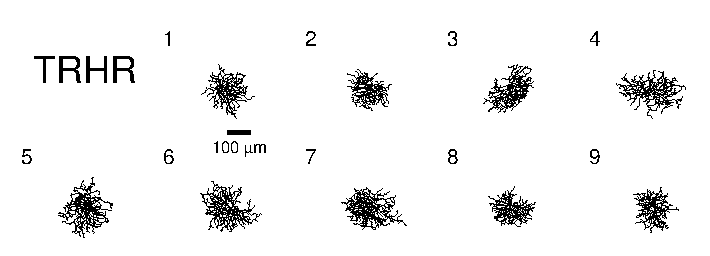
\includegraphics[scale=1.5]{Figures/SupFig1/TRHR-all-cells-1.eps}}
  \caption{}
\end{figure}

\begin{table}
  \centering
  \begin{tabular}{rl}
    \toprule
    cell & file \\
    \midrule
1& \url{P32TRHR-02232012-A1R1-40x-stitch} \\
2& \url{P34TRHR-02242012-R1C2-40x} \\
3& \url{P40-TRHR-03222012-r2c2-40x} \\
4& \url{TRHR-07182012-a1r1-cell1-40x-0} \\
5& \url{TRHR-07182012-a1r1-cell2-40x-0.8zoom} \\
6& \url{TRHR-07182012-a1r2-40x-08zoom} \\
7& \url{TRHR-07182012-a1r2-cell2-40x-07zoom} \\
8& \url{TRHR-r1-01252012-40x} \\
9& \url{trhr-04032012-corrected} \\
\bottomrule
  \end{tabular}
\end{table}


\clearpage


% To generate figures:
% drawAllNeuronsSide.m

\begin{figure}
  \centering
  \fbox{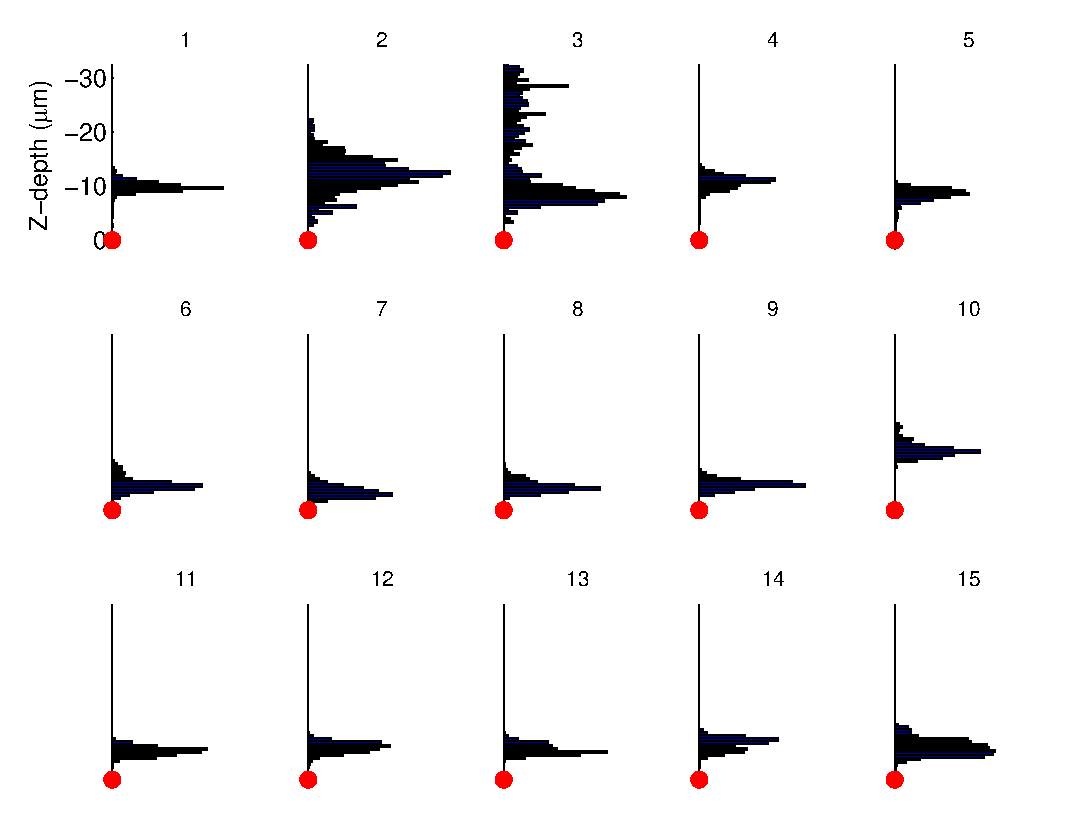
\includegraphics[scale=1]{Figures/SupFig2/CB2-stratification-depth-1}}
  \caption{}
\end{figure}

\clearpage

\begin{figure}
  \centering
  \fbox{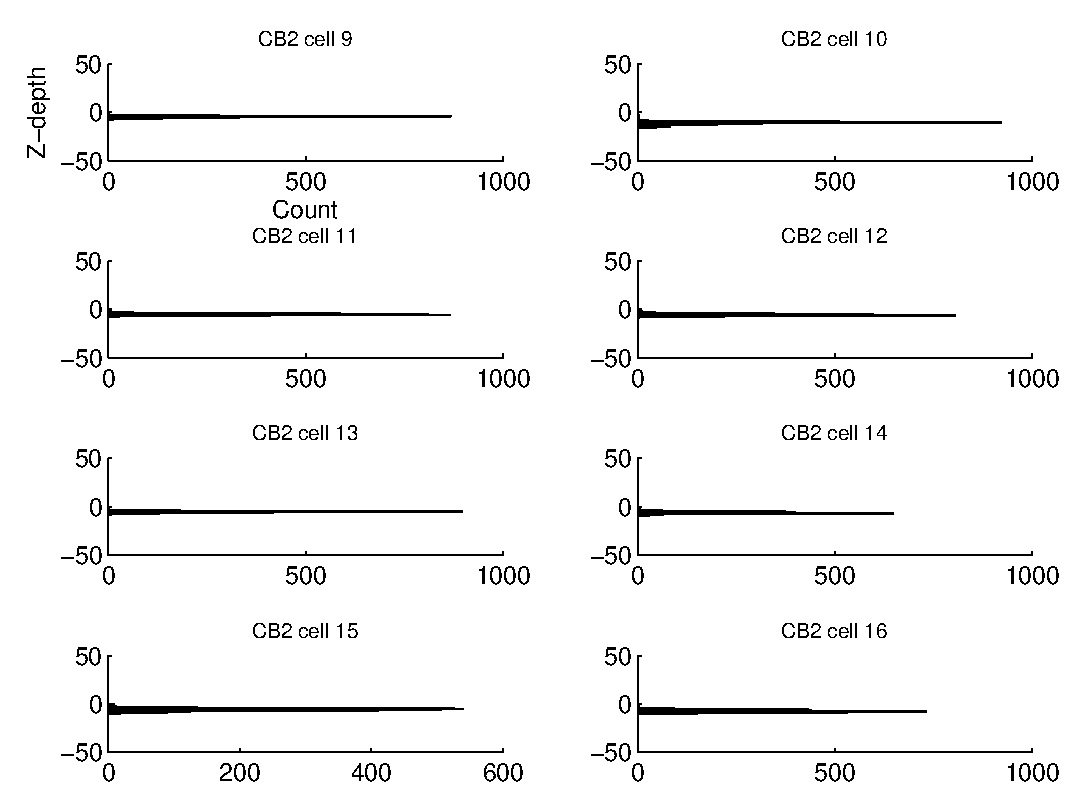
\includegraphics[scale=1]{Figures/SupFig2/CB2-stratification-depth-9}}
  \caption{}
\end{figure}

\clearpage

\begin{figure}
  \centering
  \fbox{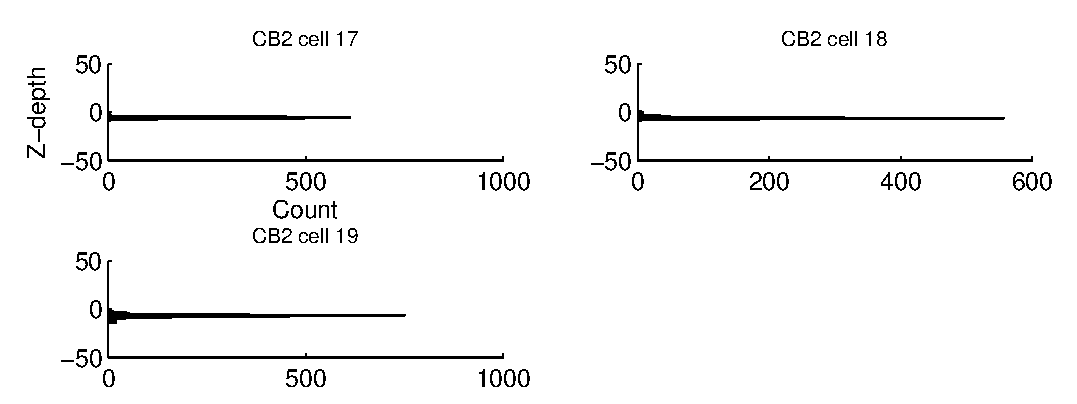
\includegraphics[scale=1]{Figures/SupFig2/CB2-stratification-depth-17}}
  \caption{}
\end{figure}

\clearpage

\begin{figure}
  \centering
  \fbox{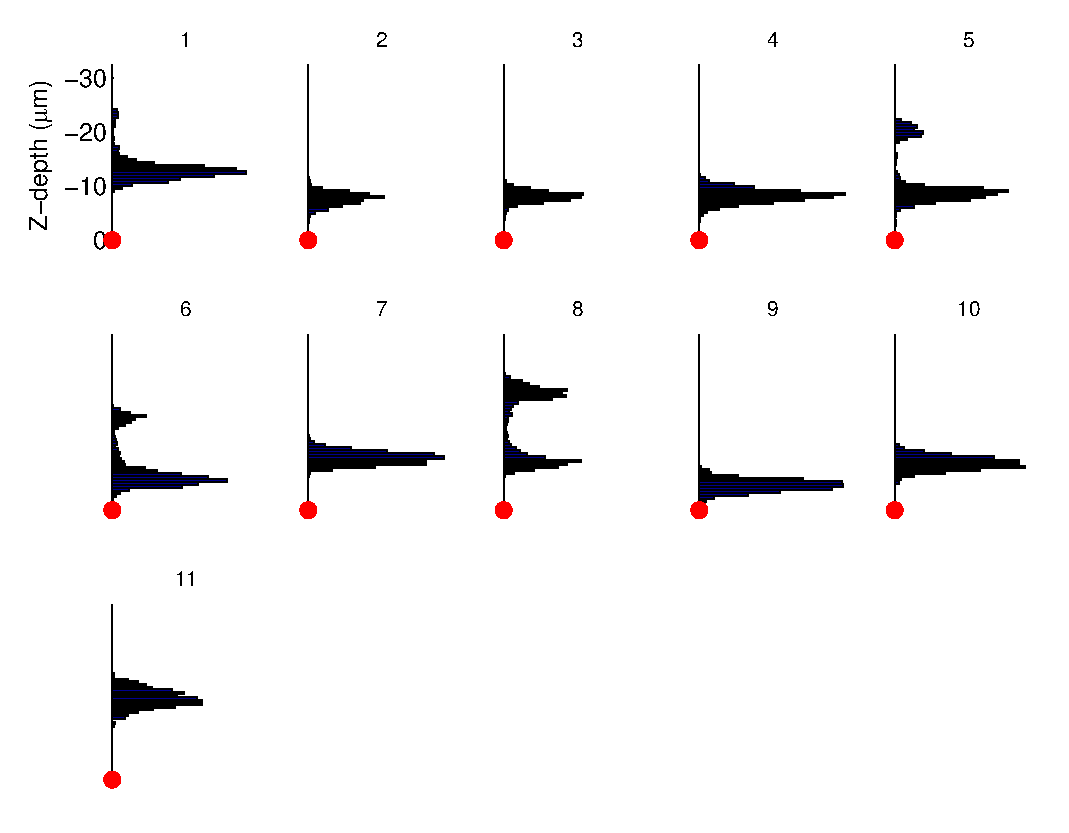
\includegraphics[scale=1]{Figures/SupFig2/Cdh3-stratification-depth-1}}
  \caption{}
\end{figure}

\clearpage

\begin{figure}
  \centering
  \fbox{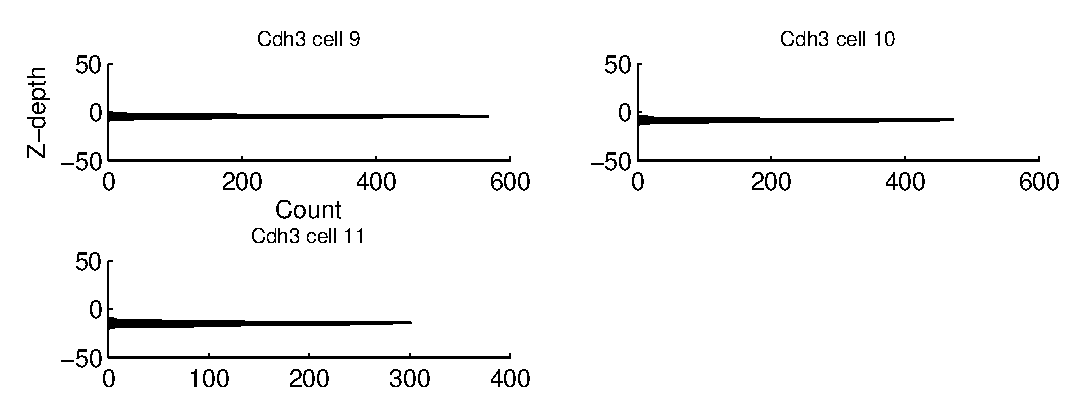
\includegraphics[scale=1]{Figures/SupFig2/Cdh3-stratification-depth-9}}
  \caption{}
\end{figure}

\clearpage

\begin{figure}
  \centering
  \fbox{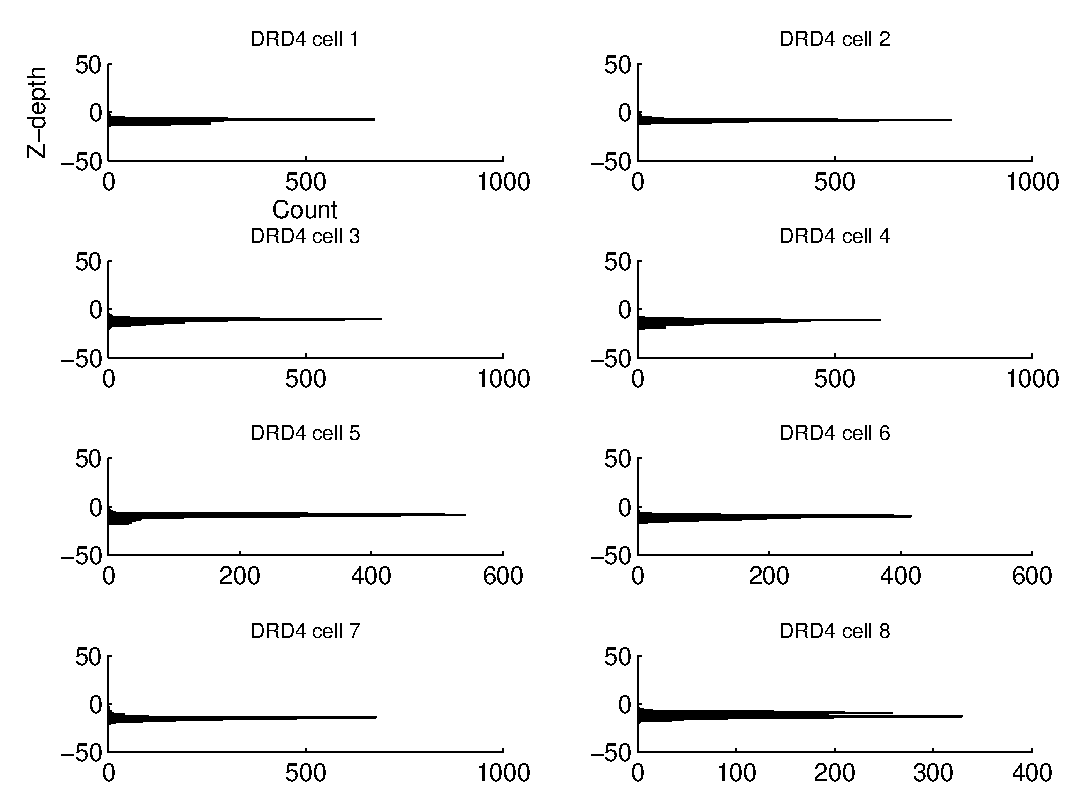
\includegraphics[scale=1]{Figures/SupFig2/DRD4-stratification-depth-1}}
  \caption{}
\end{figure}

\clearpage

\begin{figure}
  \centering
  \fbox{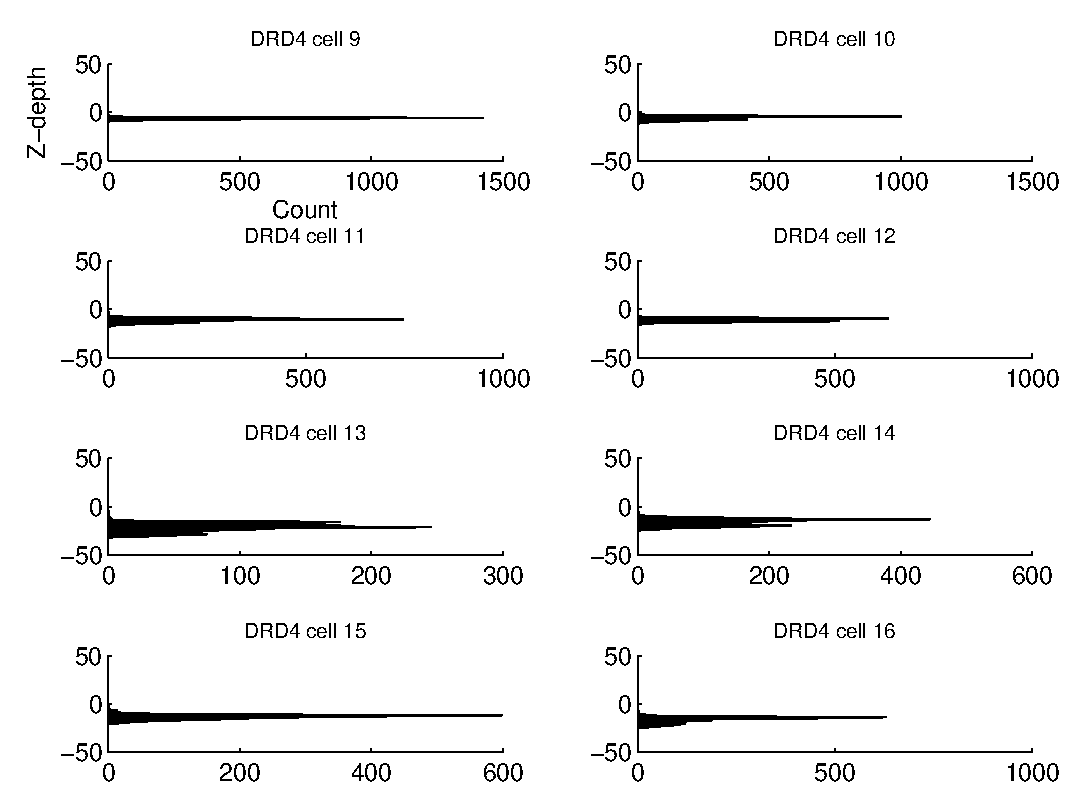
\includegraphics[scale=1]{Figures/SupFig2/DRD4-stratification-depth-9}}
  \caption{}
\end{figure}

\clearpage

\begin{figure}
  \centering
  \fbox{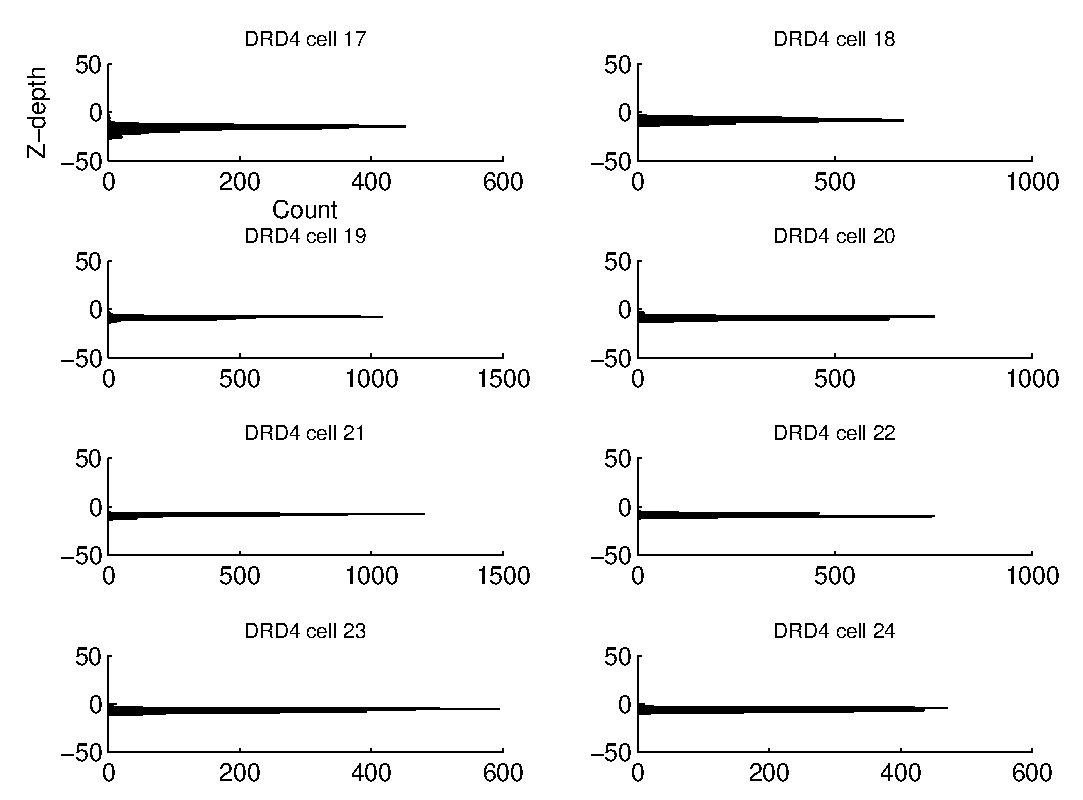
\includegraphics[scale=1]{Figures/SupFig2/DRD4-stratification-depth-17}}
  \caption{}
\end{figure}

\clearpage

\begin{figure}
  \centering
  \fbox{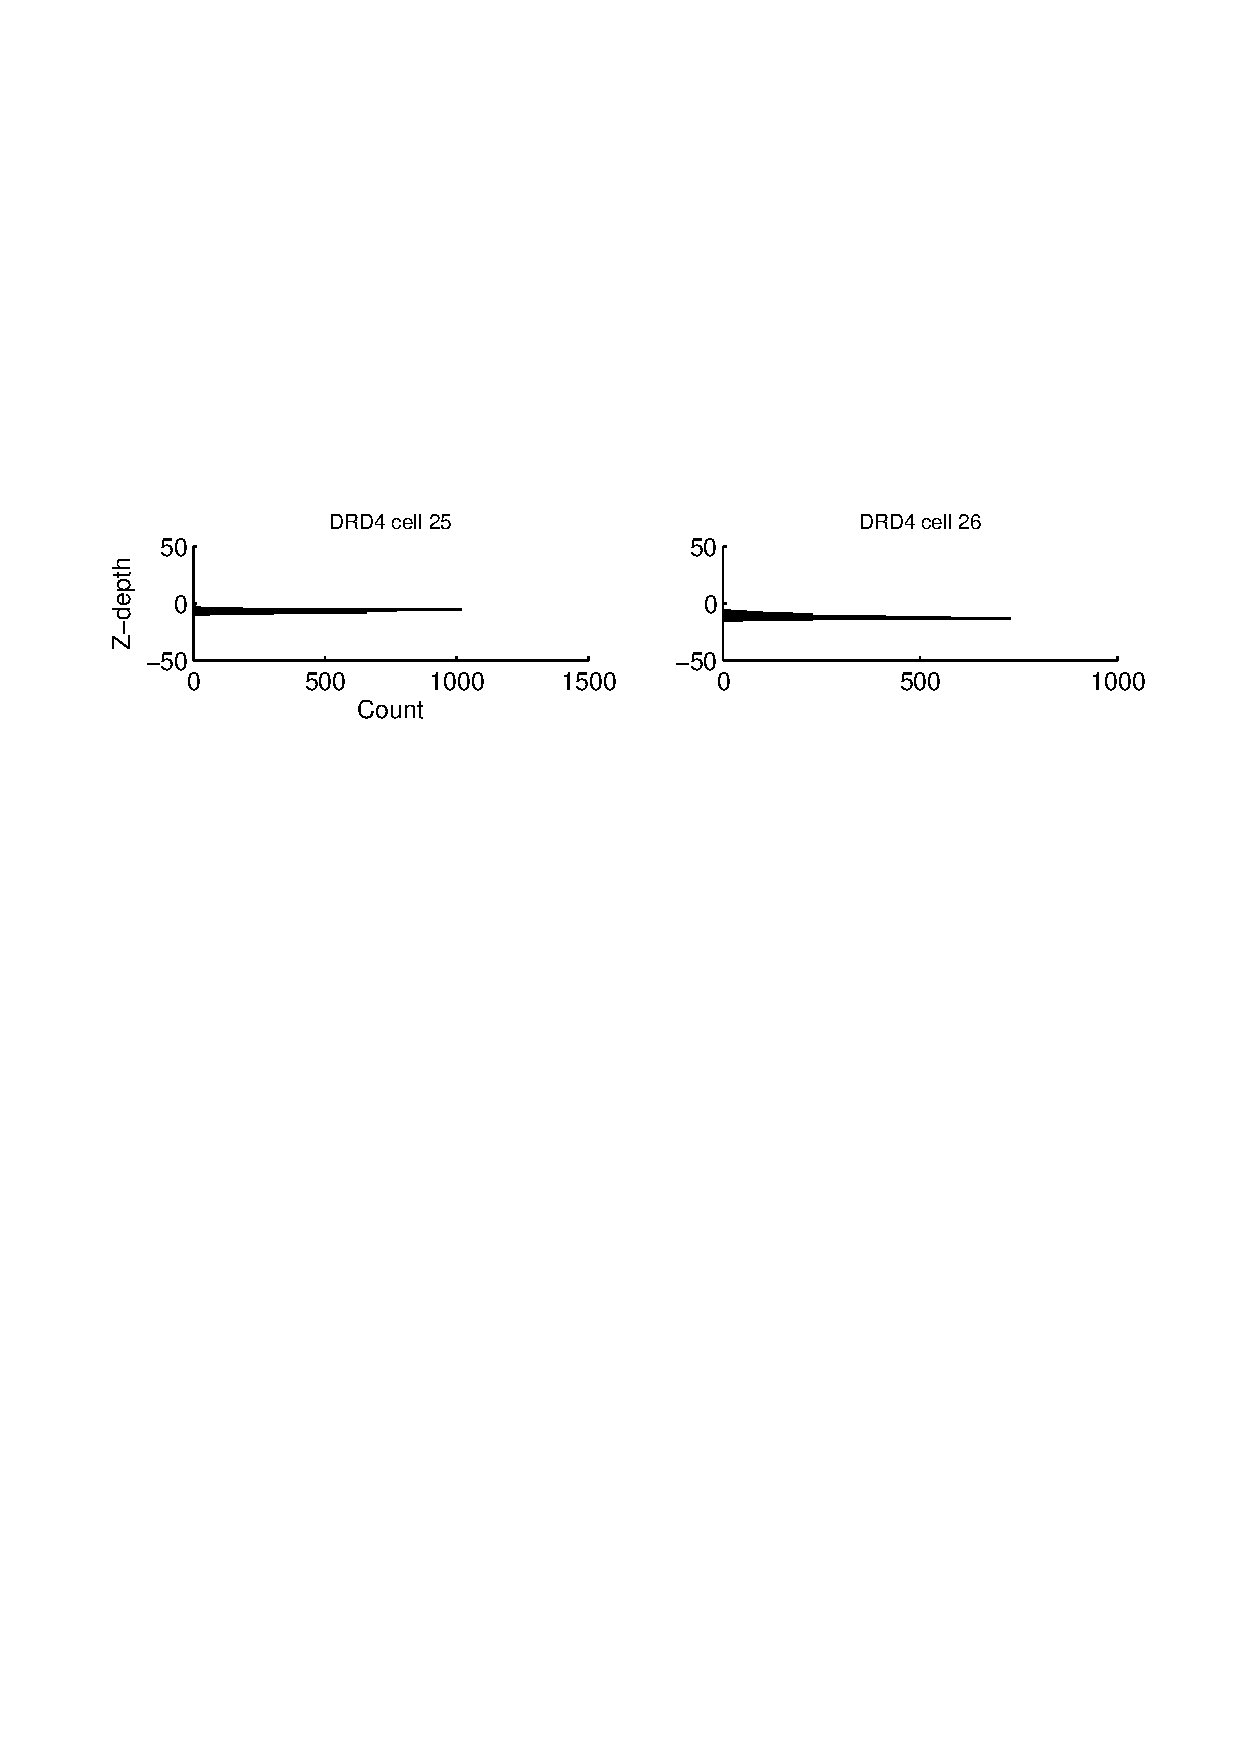
\includegraphics[scale=1]{Figures/SupFig2/DRD4-stratification-depth-25}}
  \caption{}
\end{figure}

\clearpage

\begin{figure}
  \centering
  \fbox{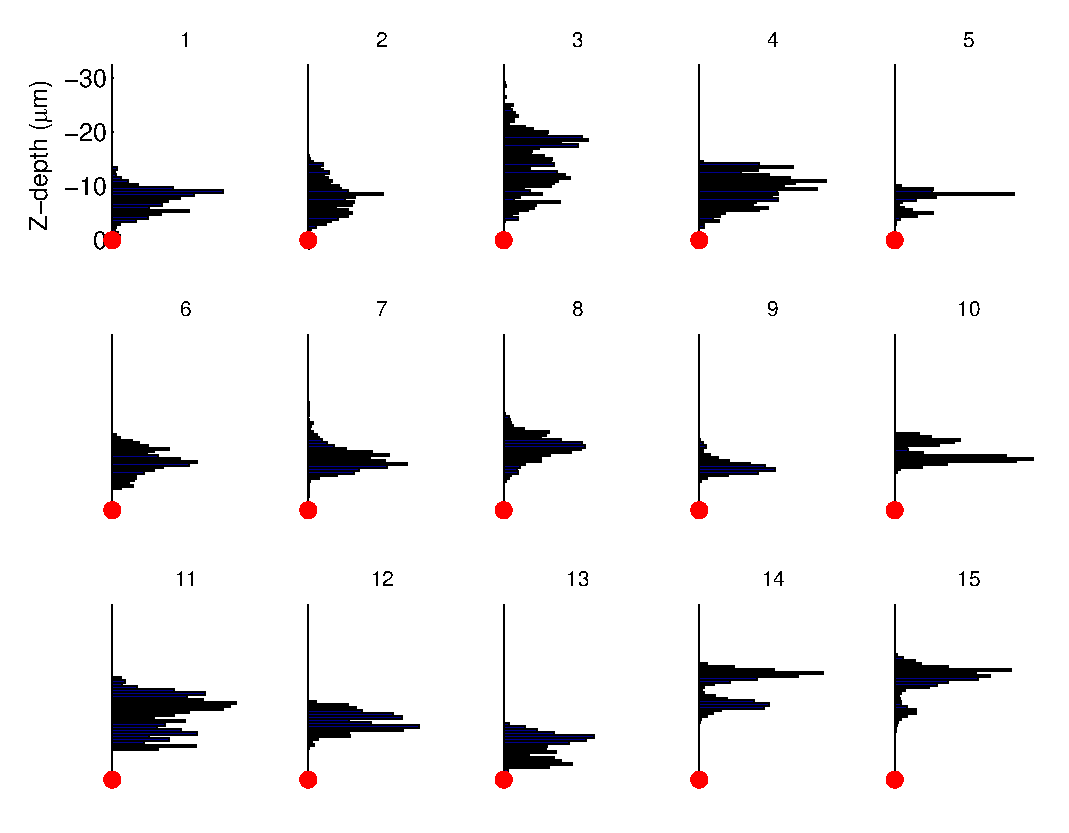
\includegraphics[scale=1]{Figures/SupFig2/Hoxd10-stratification-depth-1}}
  \caption{}
\end{figure}

\clearpage

\begin{figure}
  \centering
  \fbox{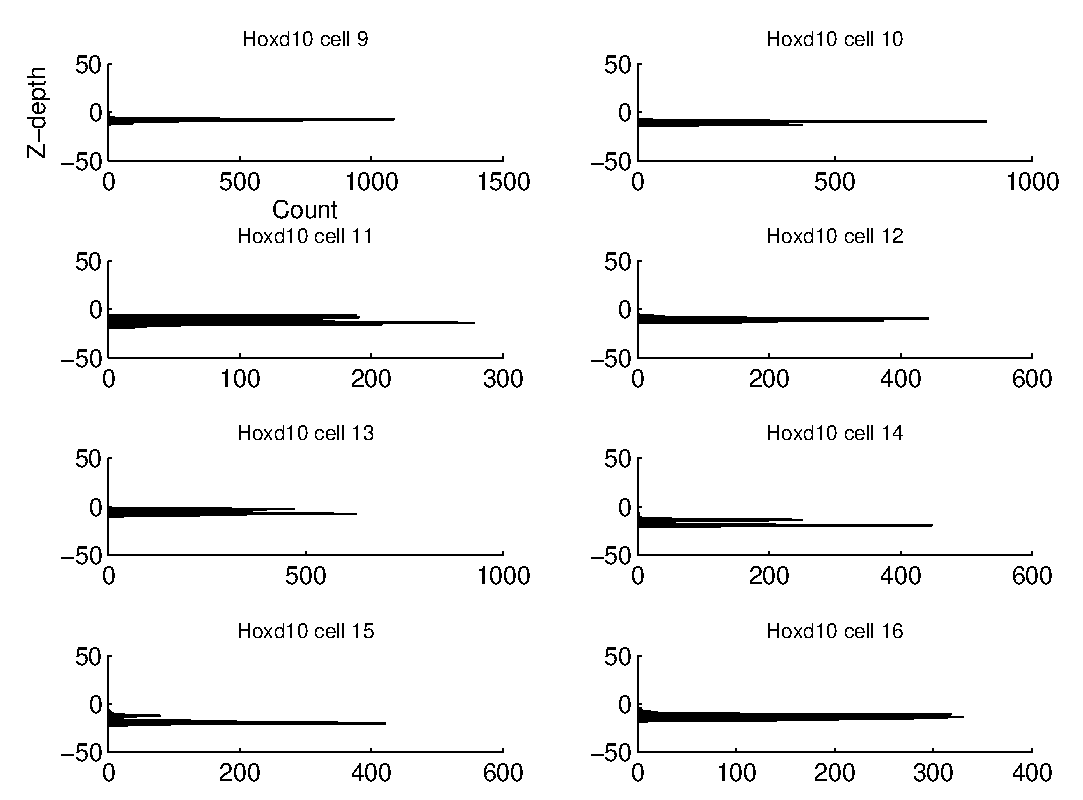
\includegraphics[scale=1]{Figures/SupFig2/Hoxd10-stratification-depth-9}}
  \caption{}
\end{figure}

\clearpage

\begin{figure}
  \centering
  \fbox{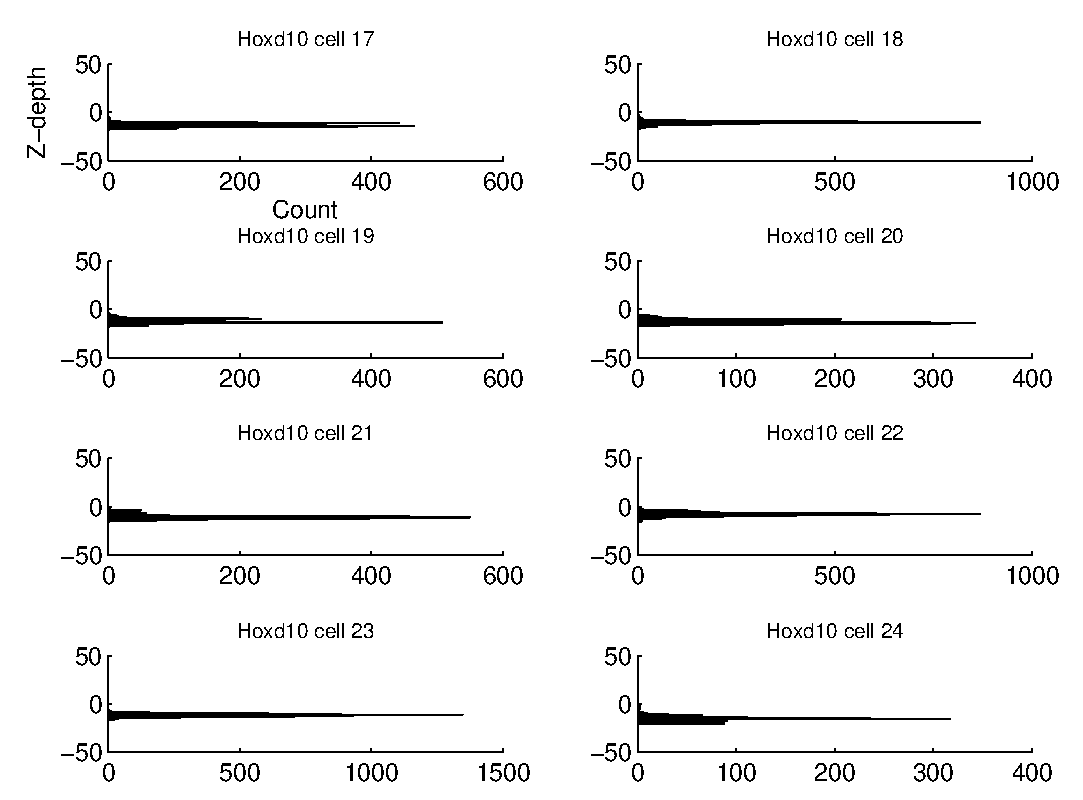
\includegraphics[scale=1]{Figures/SupFig2/Hoxd10-stratification-depth-17}}
  \caption{}
\end{figure}

\clearpage

\begin{figure}
  \centering
  \fbox{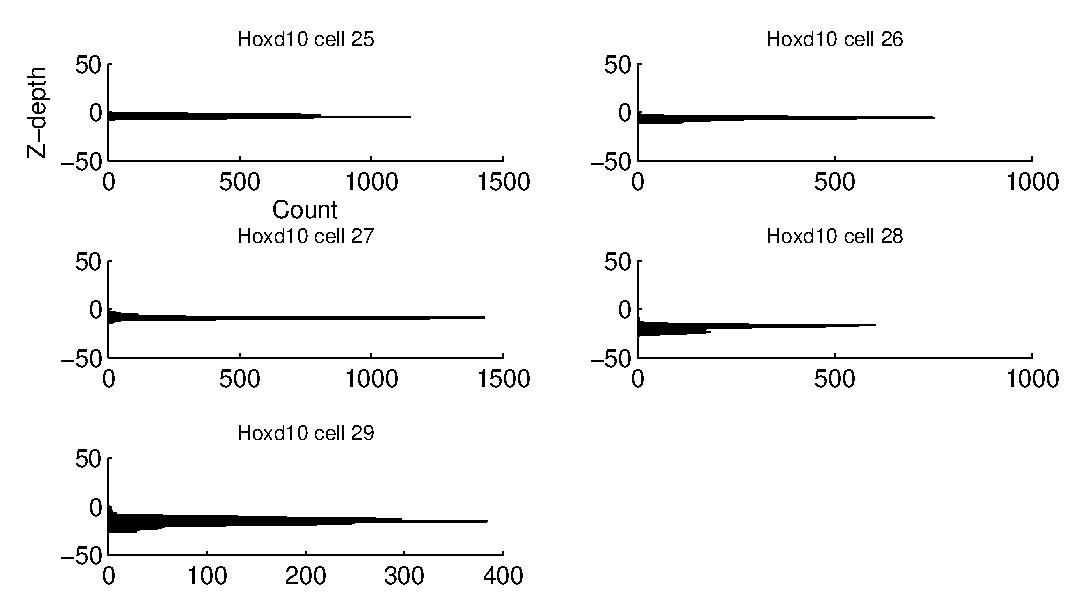
\includegraphics[scale=1]{Figures/SupFig2/Hoxd10-stratification-depth-25}}
  \caption{}
\end{figure}

\clearpage

\begin{figure}
  \centering
  \fbox{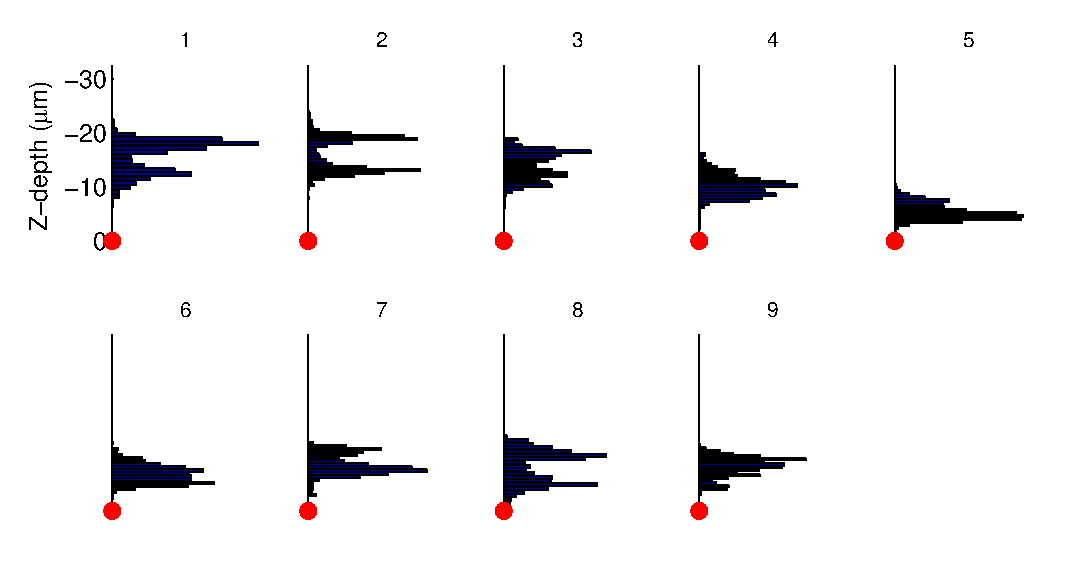
\includegraphics[scale=1]{Figures/SupFig2/TRHR-stratification-depth-1}}
  \caption{}
\end{figure}

\clearpage

\begin{figure}
  \centering
  \fbox{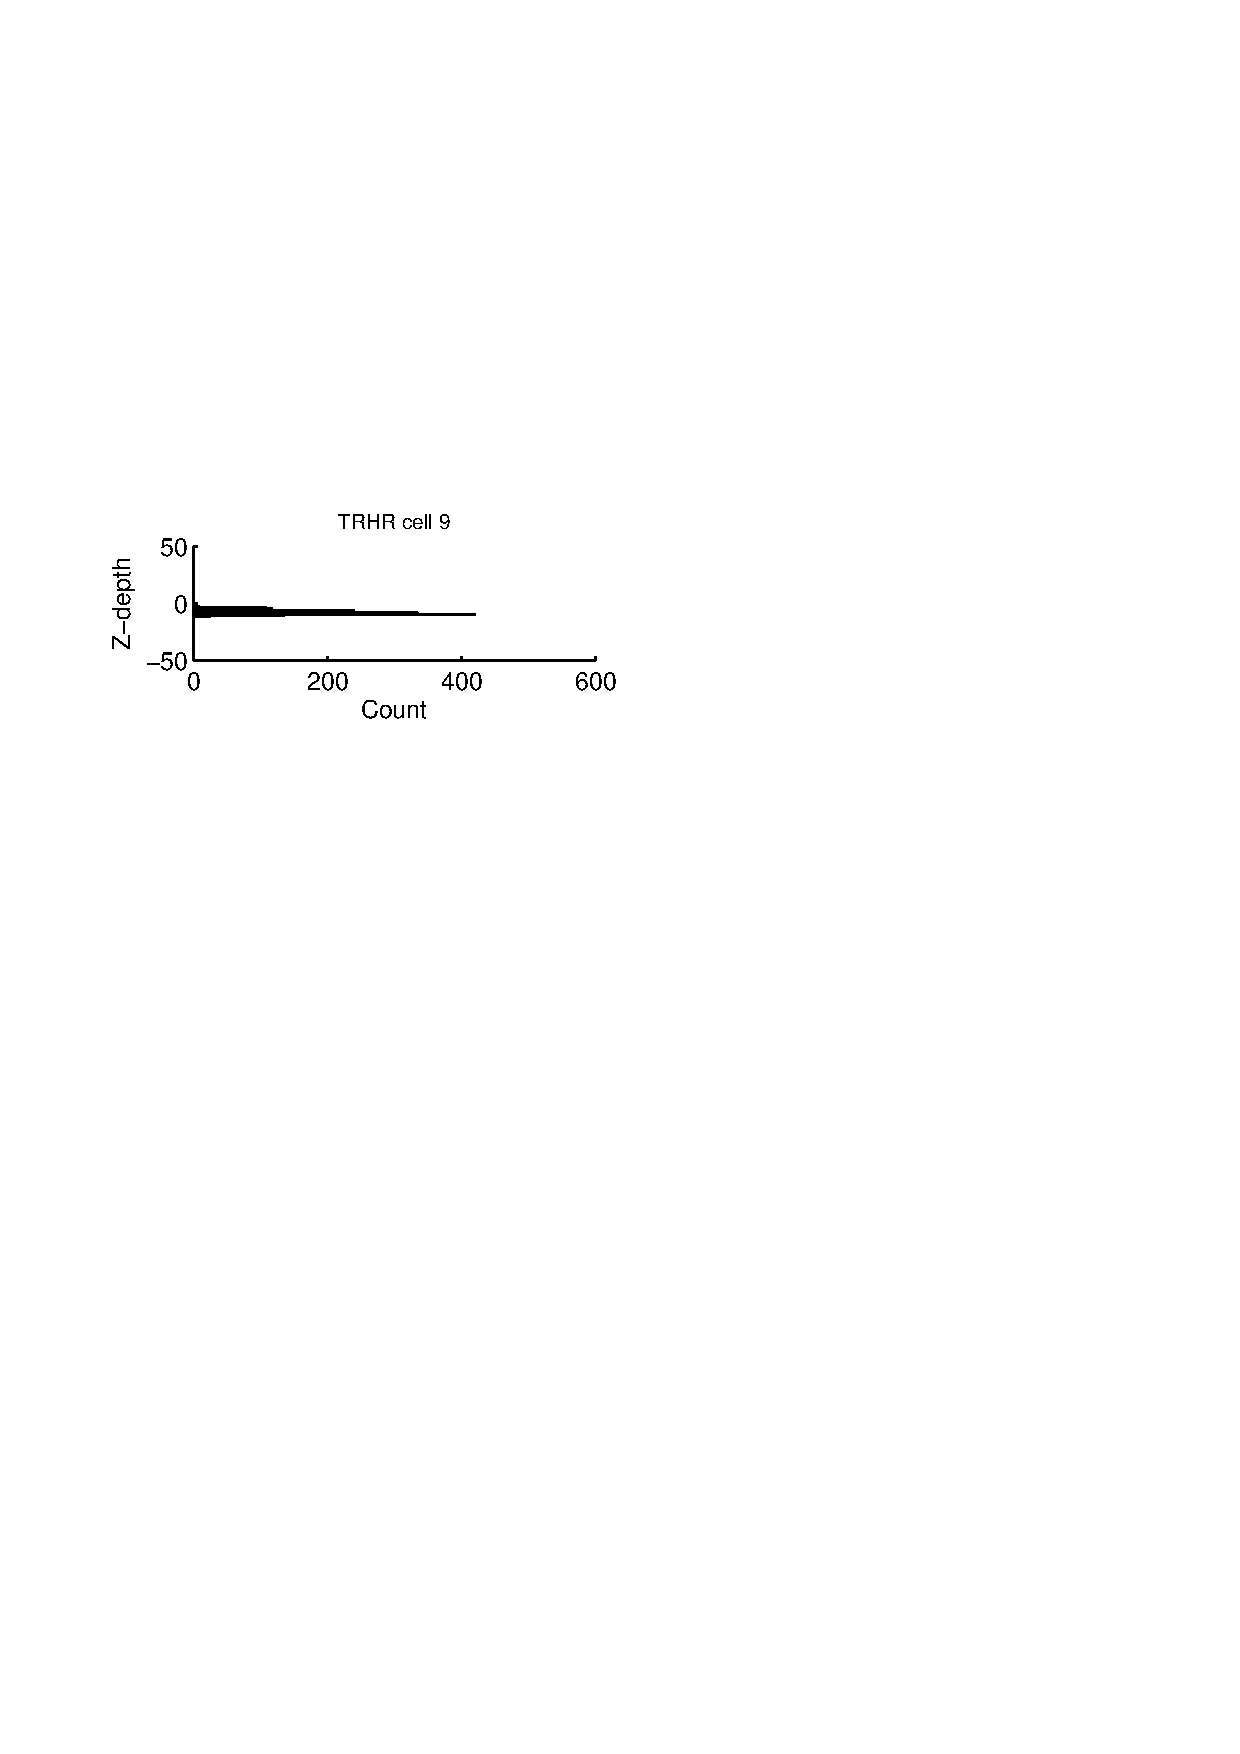
\includegraphics[scale=1]{Figures/SupFig2/TRHR-stratification-depth-9}}
  \caption{}
\end{figure}

\clearpage

% To generate figures:
% plotAllFeaturesForSupplementary.m

\begin{figure}
  \centering
  \fbox{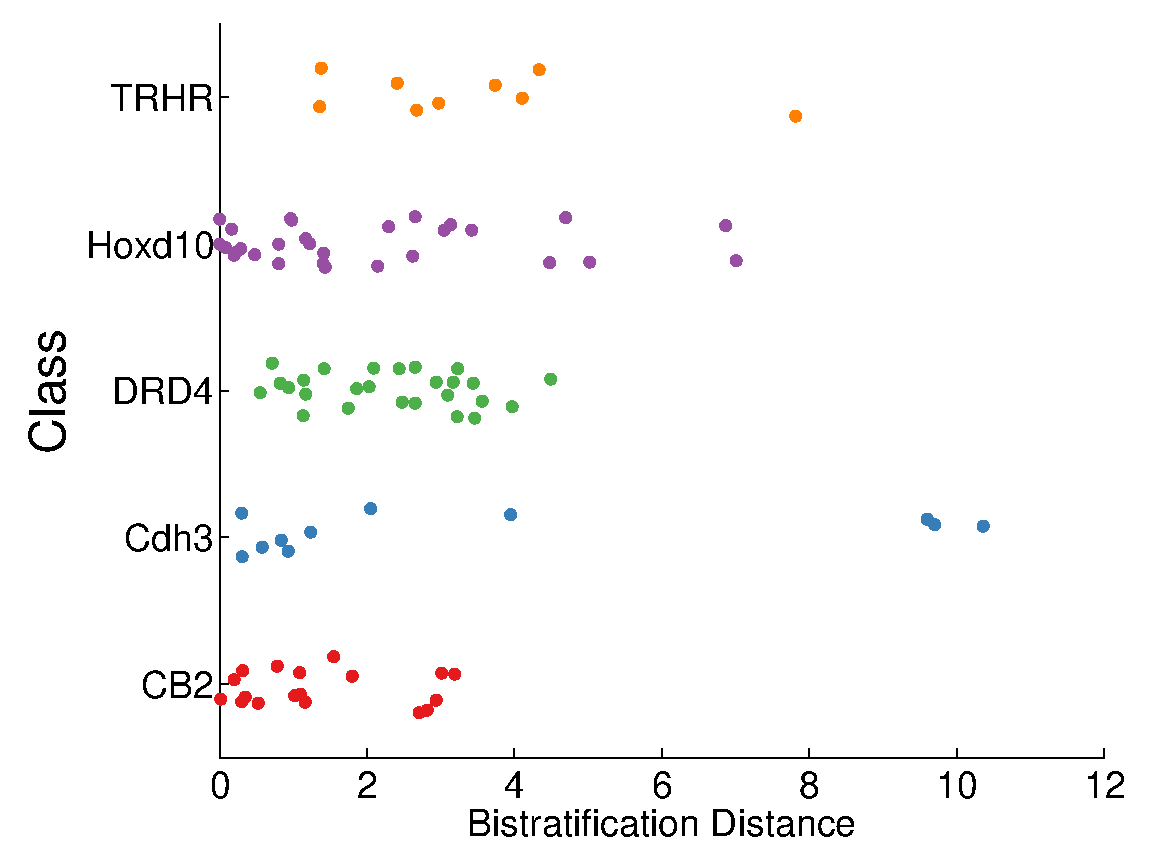
\includegraphics[scale=0.5]{Figures/SupFig3/plotFeatures-biStratificationDistance.eps}}
  \fbox{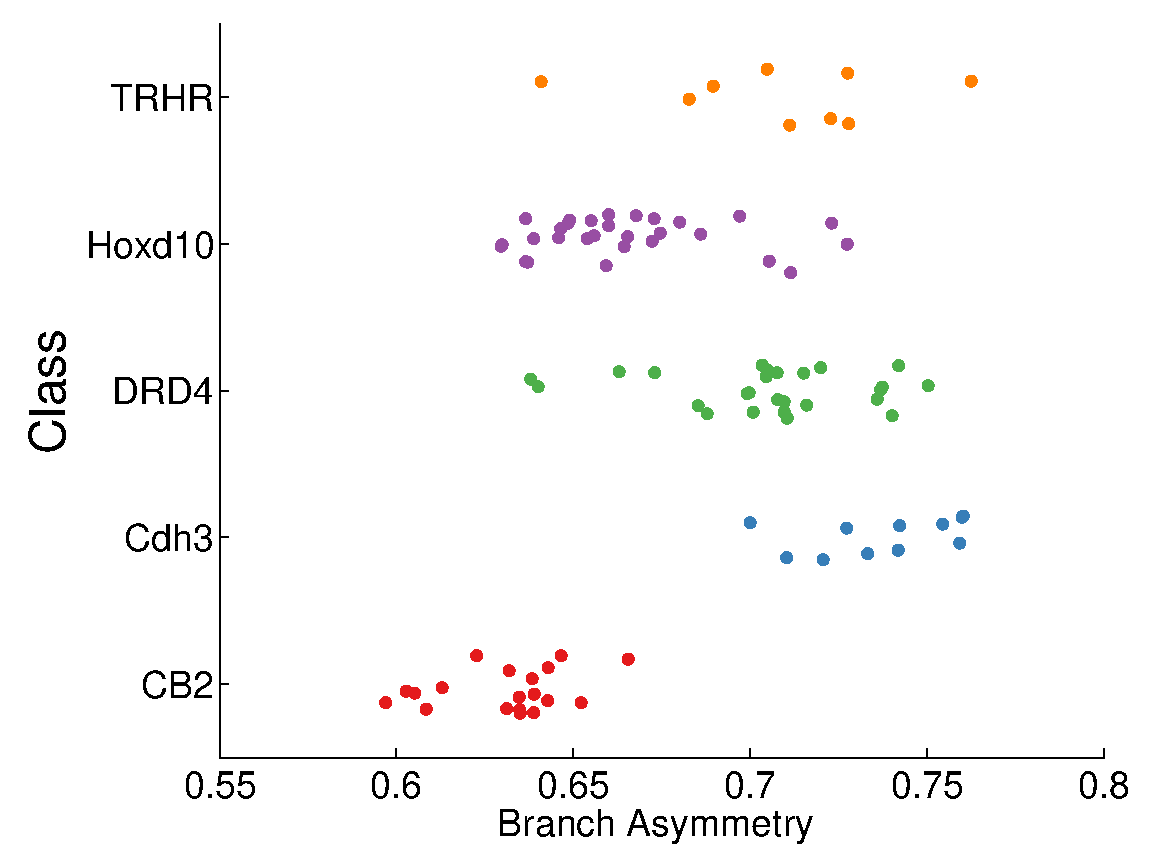
\includegraphics[scale=0.5]{Figures/SupFig3/plotFeatures-branchAssymetry.eps}}
  \fbox{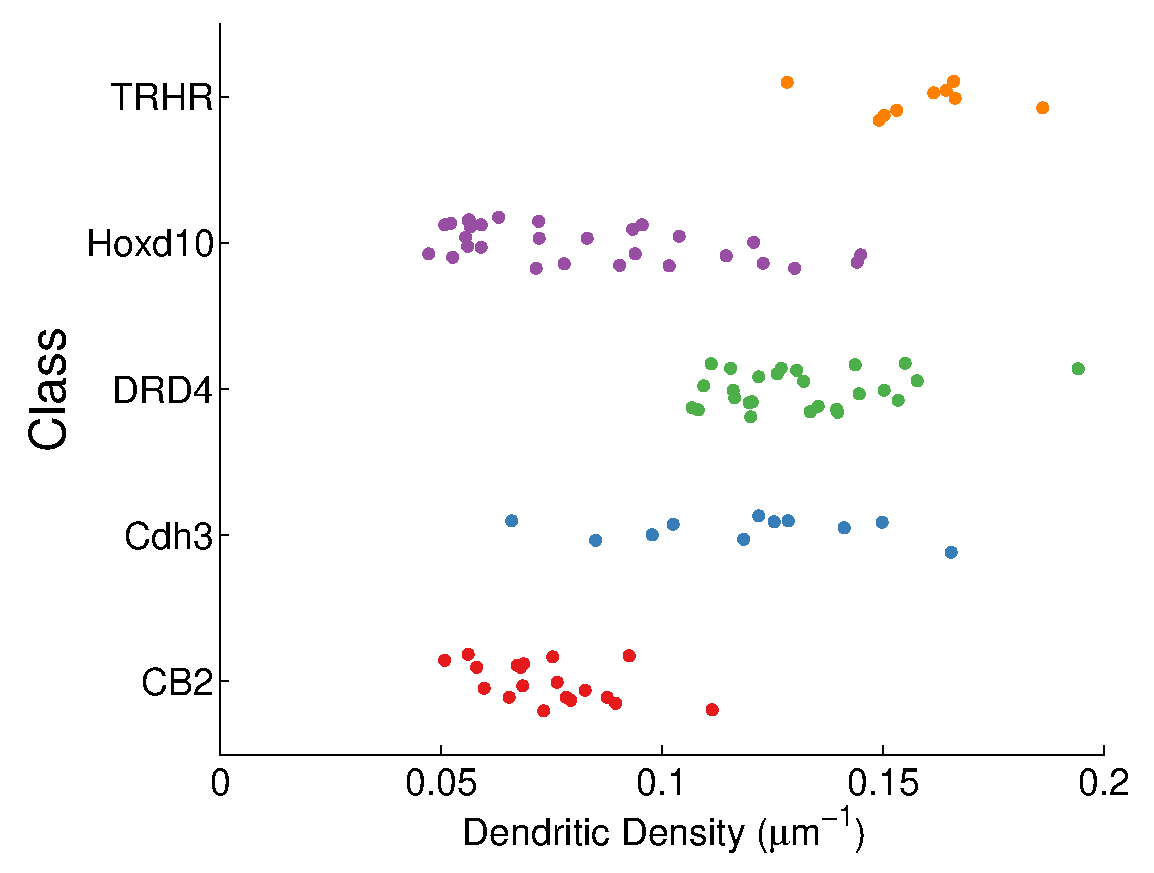
\includegraphics[scale=0.5]{Figures/SupFig3/plotFeatures-dendriticDensity.eps}}
  \caption{}
\end{figure}

\clearpage

\begin{figure}
  \centering
  \fbox{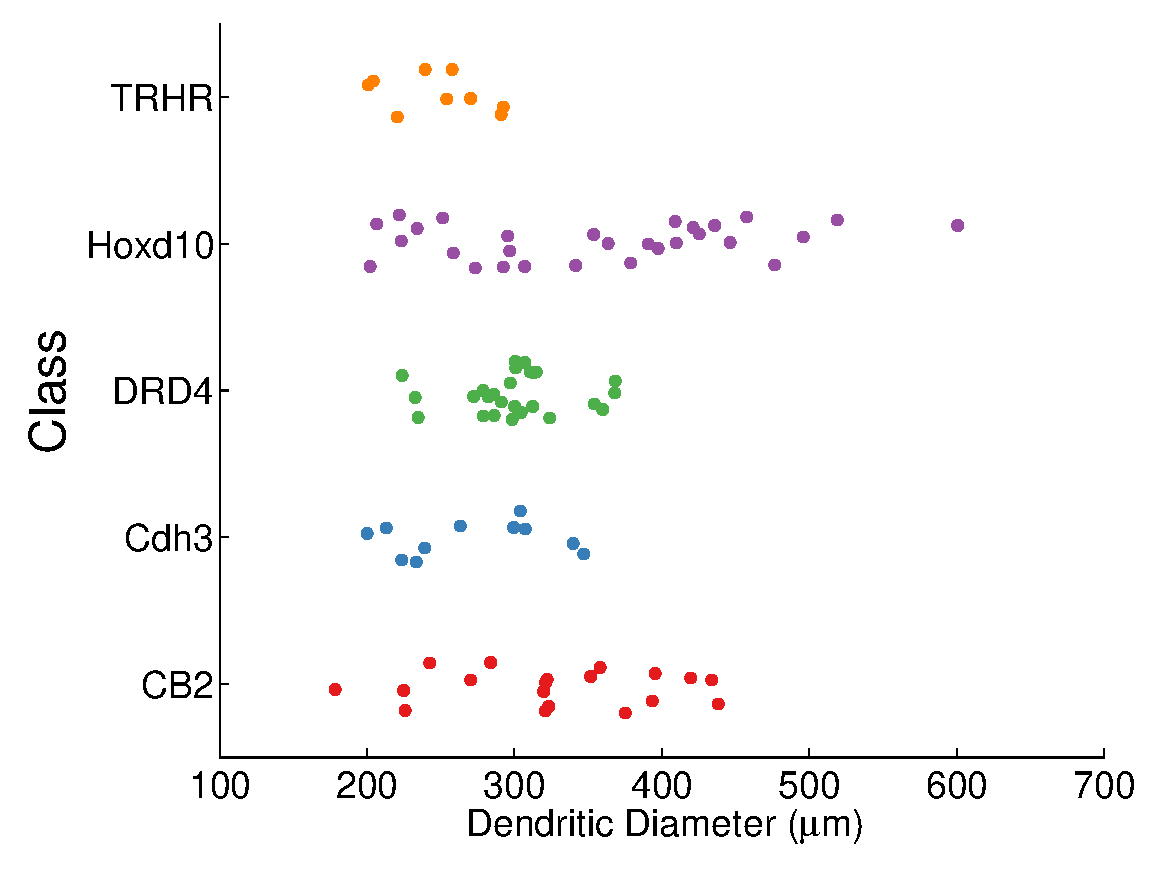
\includegraphics[scale=0.5]{Figures/SupFig3/plotFeatures-dendriticDiameter.eps}}
  \fbox{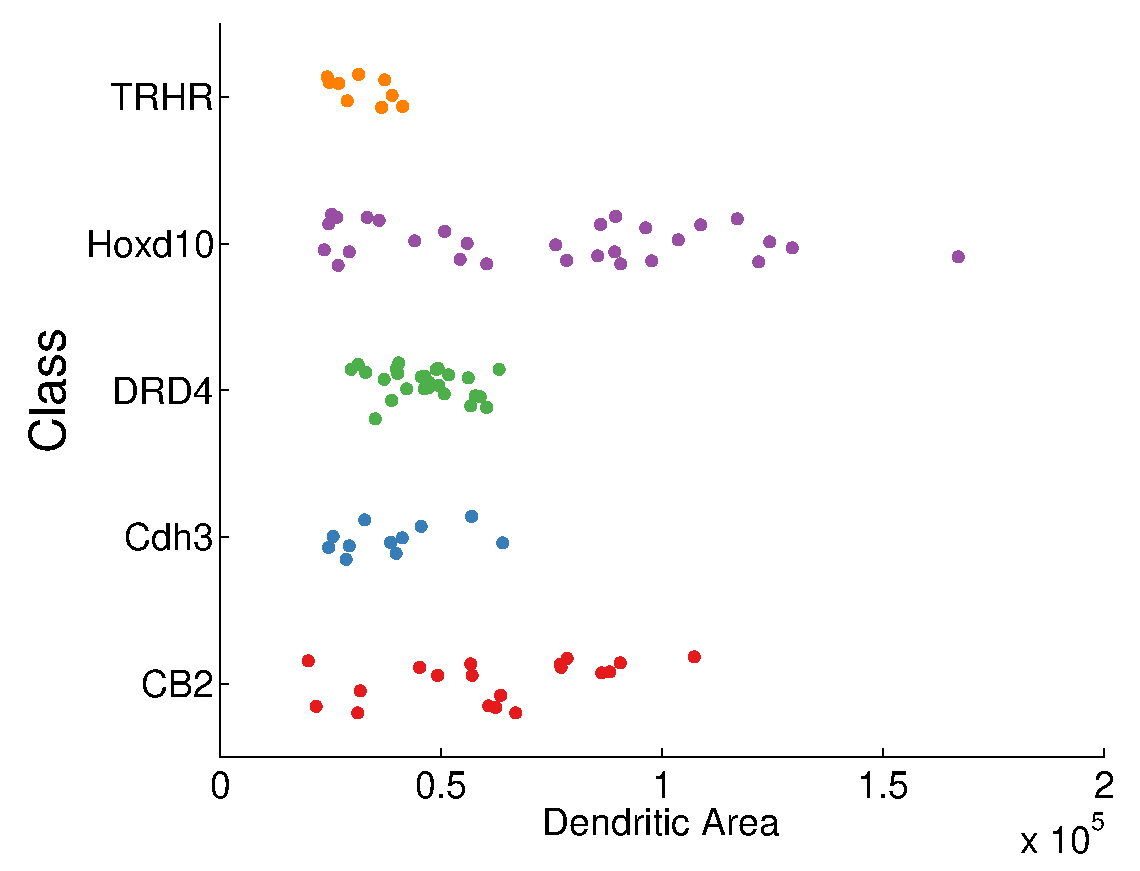
\includegraphics[scale=0.5]{Figures/SupFig3/plotFeatures-dendriticField.eps}}
  \fbox{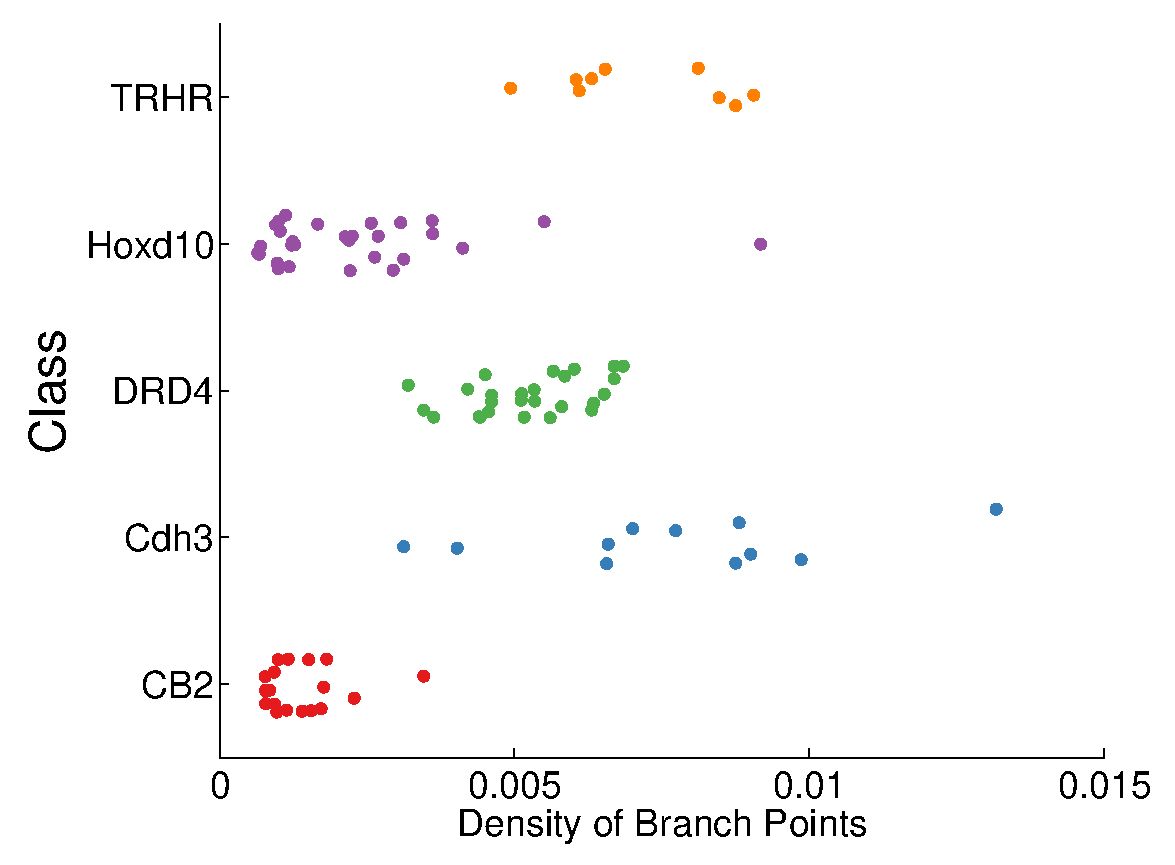
\includegraphics[scale=0.5]{Figures/SupFig3/plotFeatures-densityOfBranchPoints.eps}}
  \caption{}
\end{figure}

\clearpage

\begin{figure}
  \centering
  \fbox{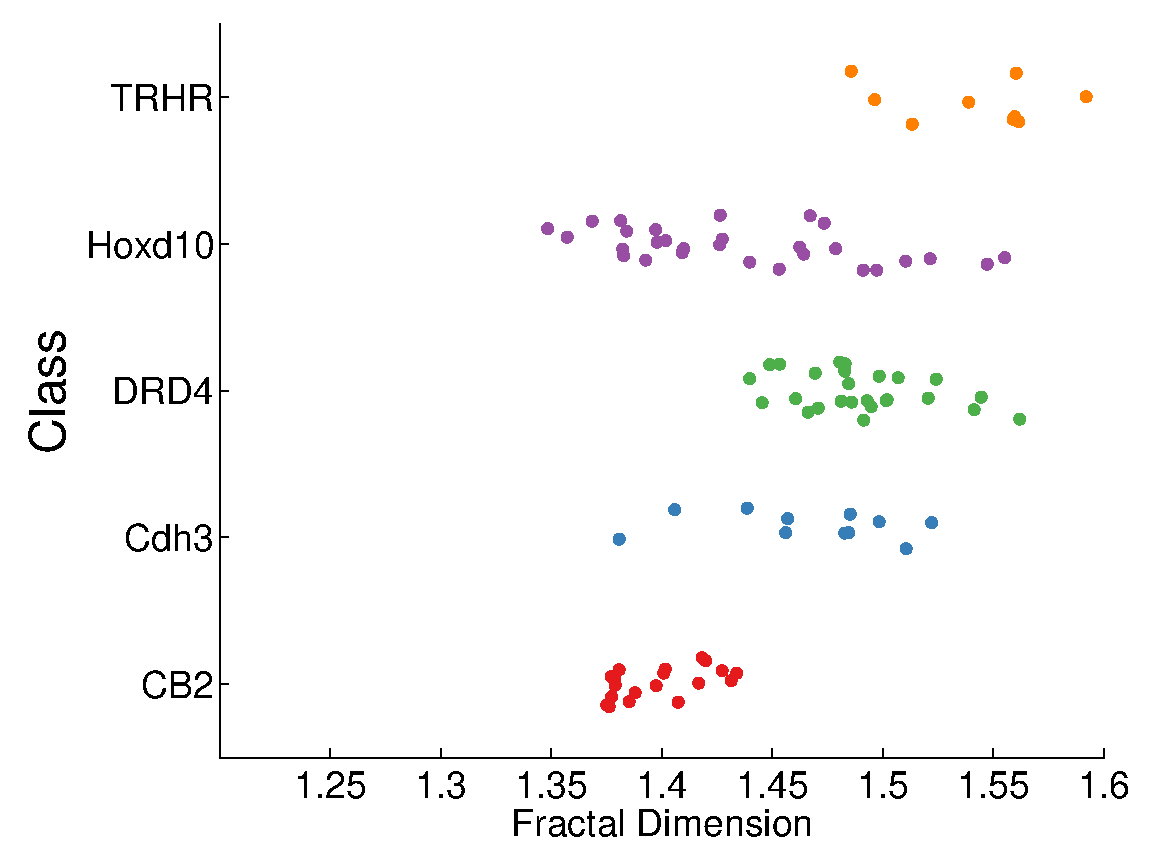
\includegraphics[scale=0.5]{Figures/SupFig3/plotFeatures-fractalDimensionBoxCounting.eps}}
  \fbox{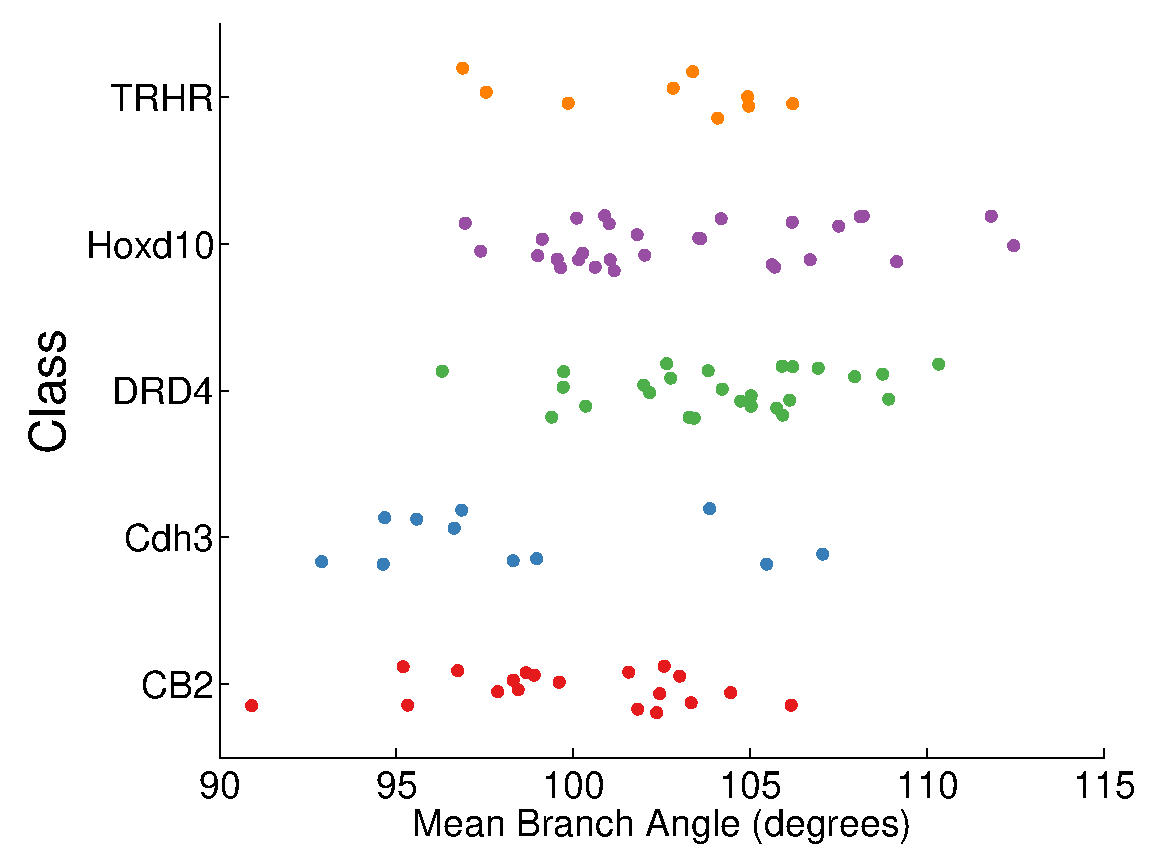
\includegraphics[scale=0.5]{Figures/SupFig3/plotFeatures-meanBranchAngle.eps}}
  \fbox{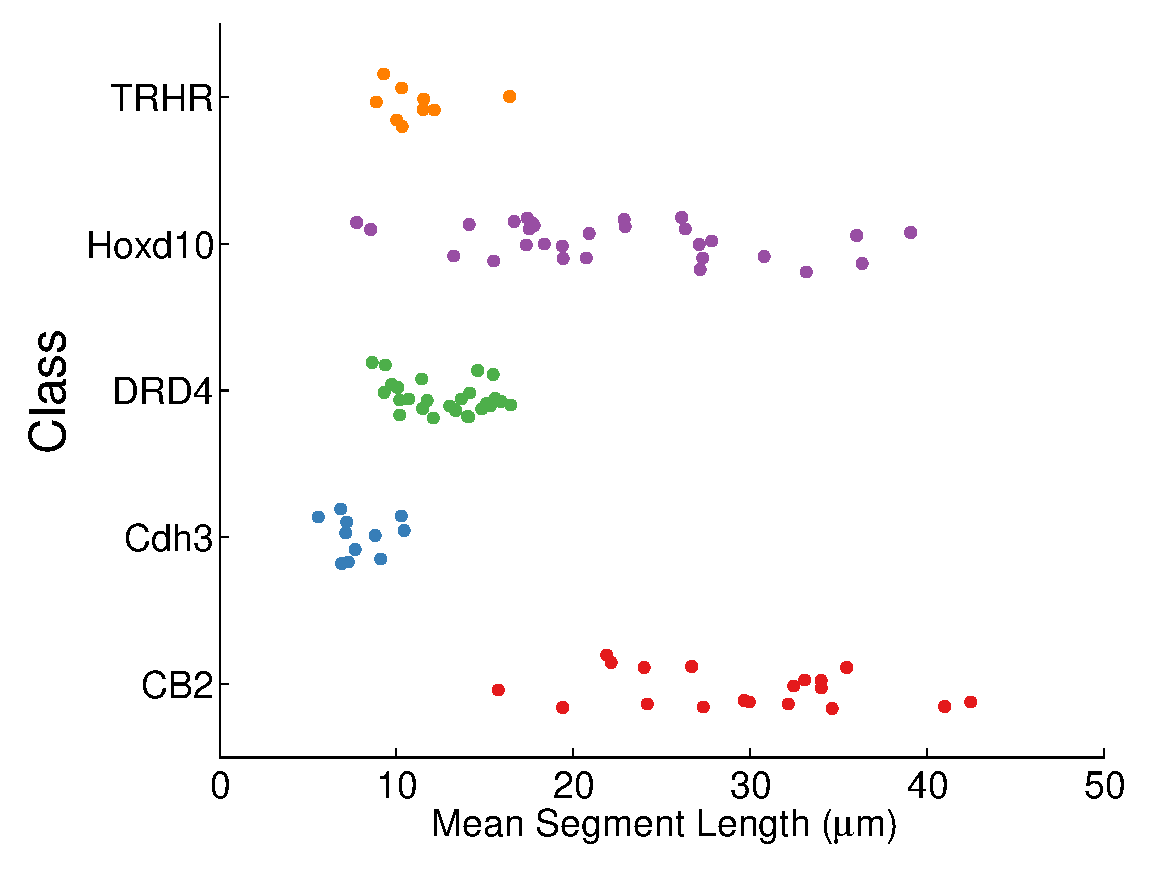
\includegraphics[scale=0.5]{Figures/SupFig3/plotFeatures-meanSegmentLength.eps}}
  \caption{}
\end{figure}

\clearpage

\begin{figure}
  \centering
  \fbox{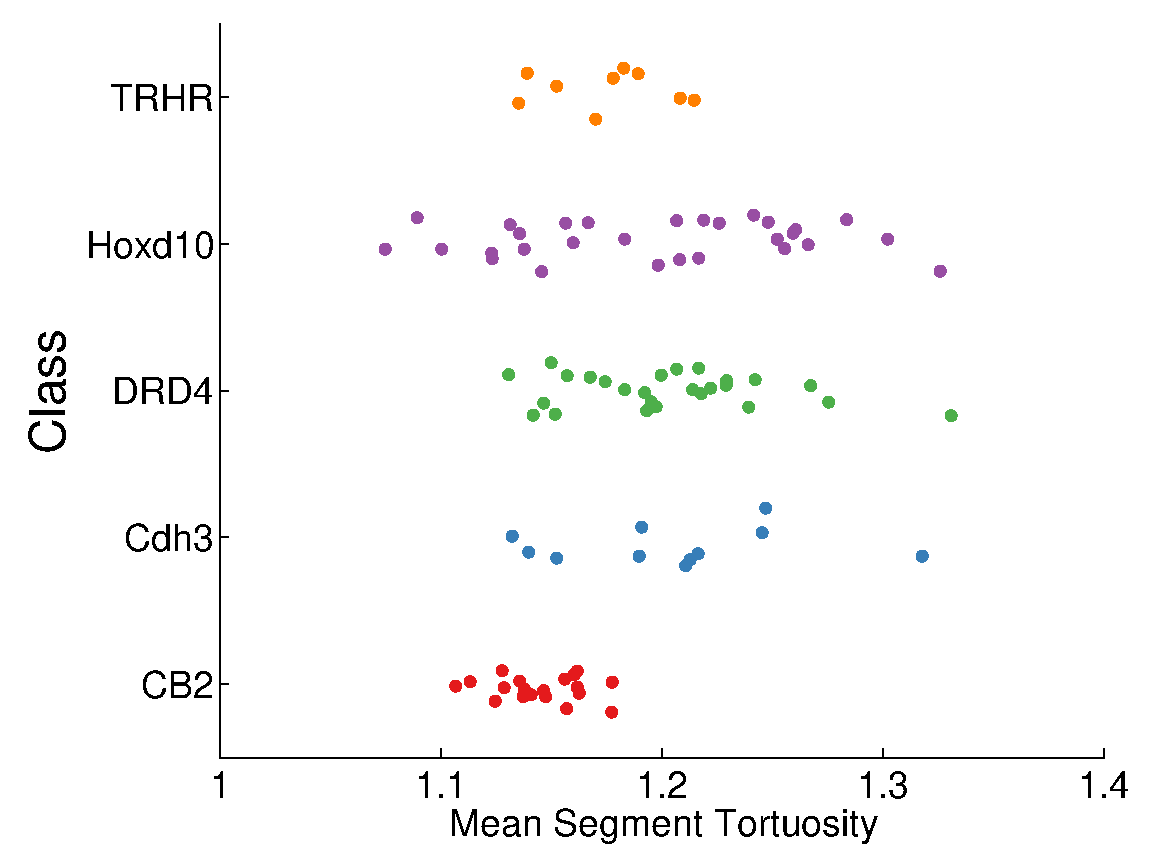
\includegraphics[scale=0.5]{Figures/SupFig3/plotFeatures-meanSegmentTortuosity.eps}}
  \fbox{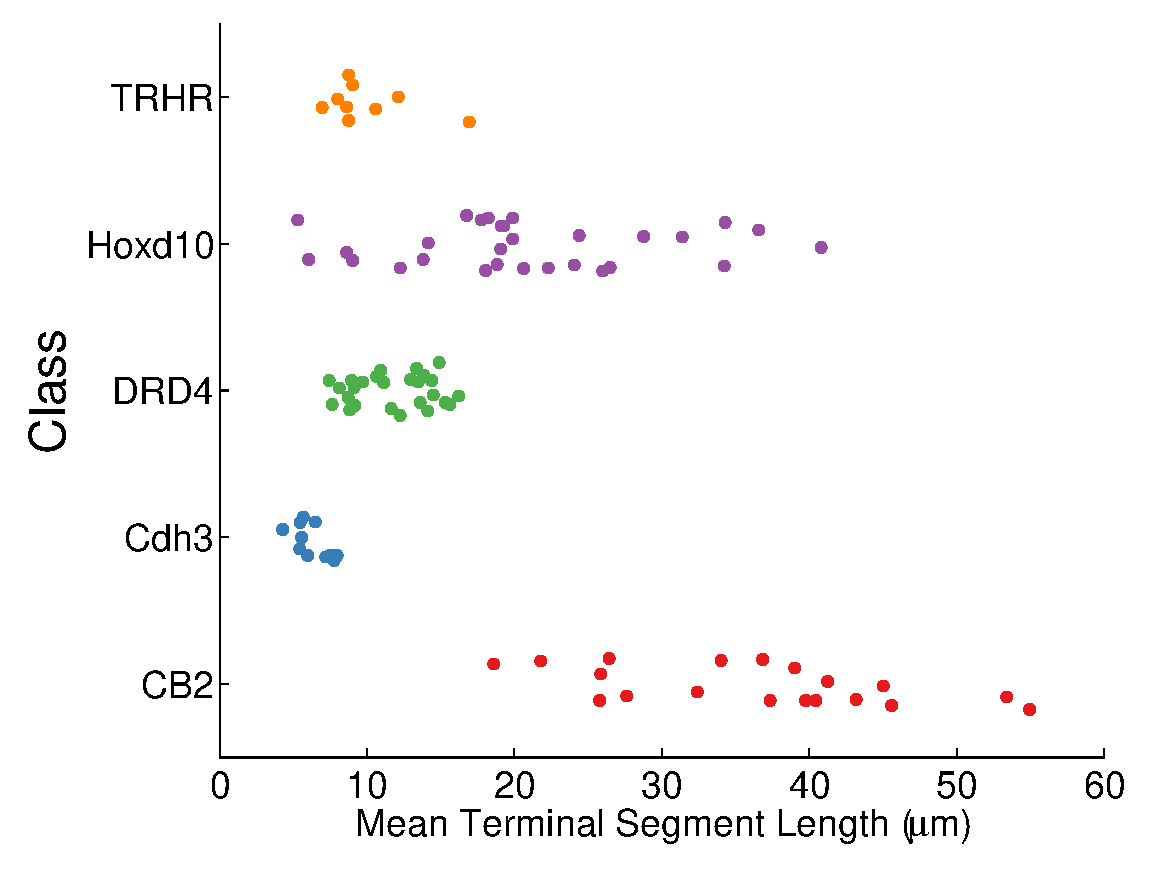
\includegraphics[scale=0.5]{Figures/SupFig3/plotFeatures-meanTerminalSegmentLength.eps}}
  \fbox{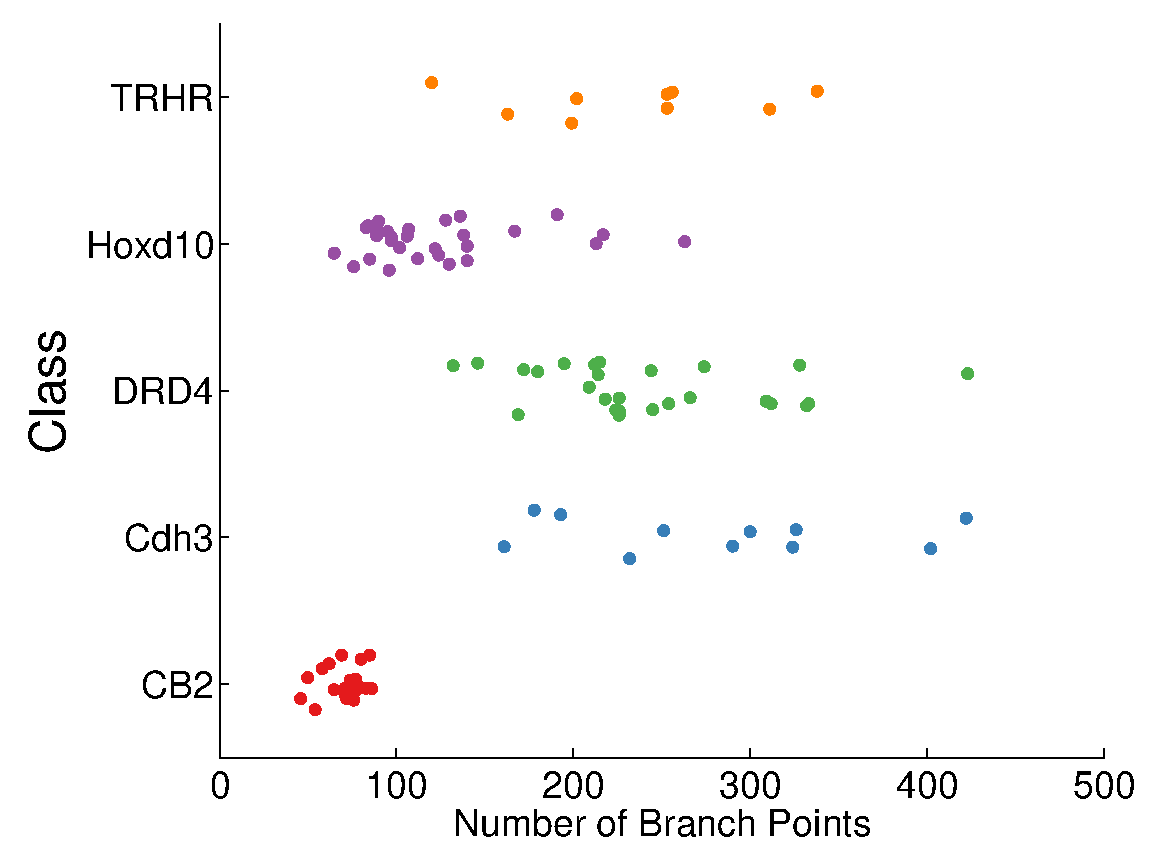
\includegraphics[scale=0.5]{Figures/SupFig3/plotFeatures-numBranchPoints.eps}}
  \caption{}
\end{figure}

\clearpage

\begin{figure}
  \centering
  \fbox{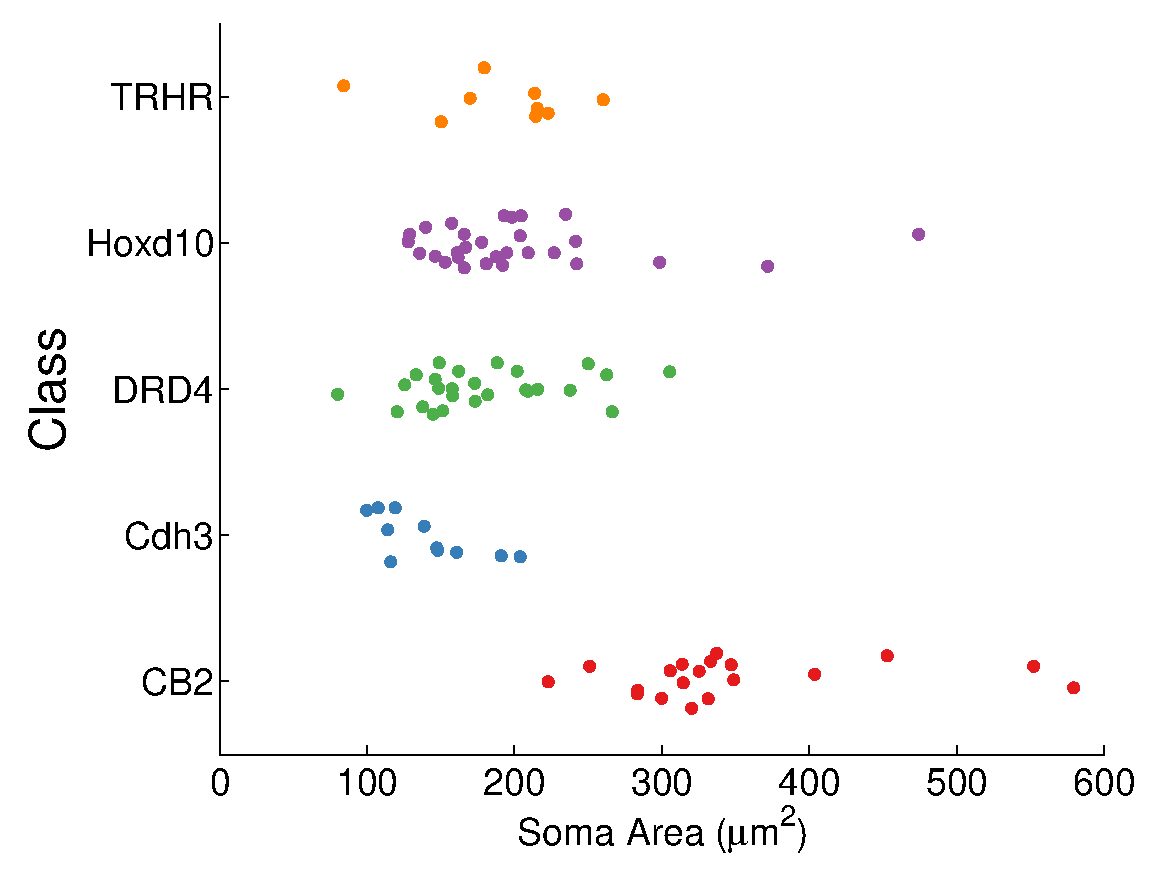
\includegraphics[scale=0.5]{Figures/SupFig3/plotFeatures-somaArea.eps}}
  \fbox{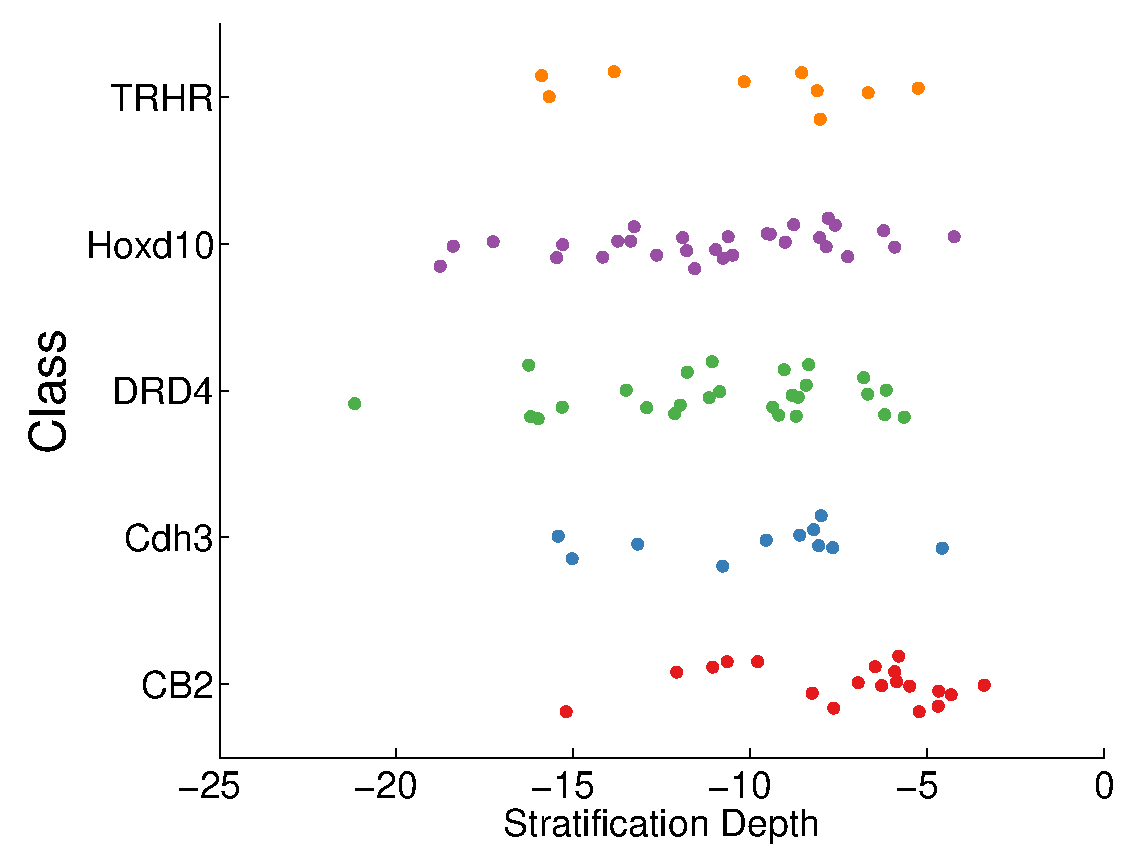
\includegraphics[scale=0.5]{Figures/SupFig3/plotFeatures-stratificationDepth.eps}}
  \fbox{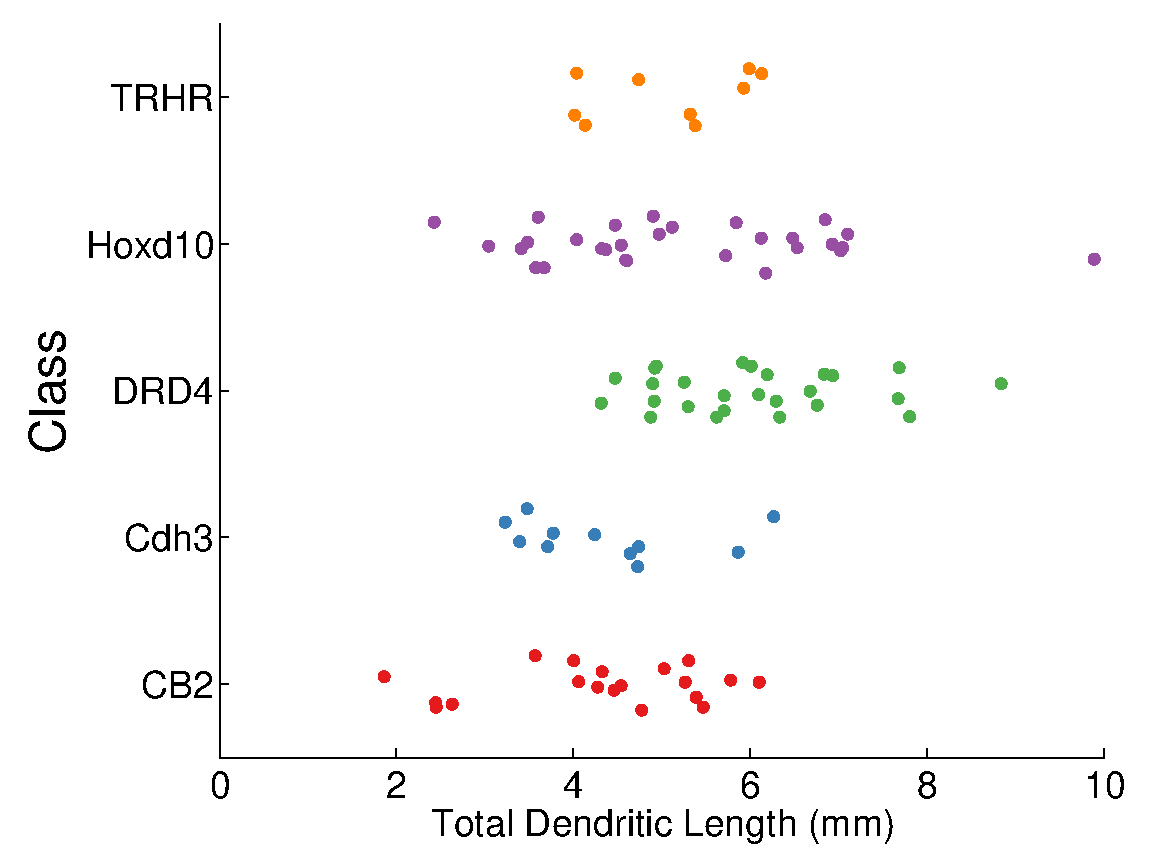
\includegraphics[scale=0.5]{Figures/SupFig3/plotFeatures-totalDendriticLength.eps}}
  \caption{}
\end{figure}

\clearpage



\end{document}
